\documentclass[12pt,a4paper]{article}
\usepackage[utf8]{inputenc}
\usepackage[spanish]{babel}
\usepackage{geometry}
\geometry{a4paper, margin=2.5cm}
\usepackage{graphicx}
\usepackage{tabularx}
\usepackage{booktabs}
\usepackage{multirow}
\usepackage{hyperref}
\usepackage[T1]{fontenc}
\usepackage{lmodern}
\usepackage[table]{xcolor}
\usepackage{float}

\hypersetup{
    colorlinks=true,
    linkcolor=black,
    urlcolor=cyan,
    citecolor=black,
}


\newcommand{\instruccion}[1]{\textcolor{red}{\textit{[#1]}}}
\newcommand{\ejemplo}[1]{\textcolor{gray}{\textit{Ejemplo: #1}}}


% --- CONFIGURACIÓN DE ENCABEZADO Y PIE DE PÁGINA ---
\usepackage{fancyhdr}
\pagestyle{fancy}
\fancyhf{} % Limpia la configuración por defecto

% Parte Superior (Encabezado)
\lhead{Universidad Técnica Federico Santa María}
\rhead{Departamento de Electrónica}

% Parte Inferior (Pie de página) - ACTUALIZADO
\lfoot{PMM}                     % Extremo izquierdo
\cfoot{\thepage}                % Centro (Número de página)
\rfoot{$2^o$ Semestre}         % Extremo derecho

% Líneas divisorias (Opcional)
\renewcommand{\headrulewidth}{0.4pt} % Línea horizontal arriba
\renewcommand{\footrulewidth}{0.4pt} % Línea horizontal abajo

\title{}
\date{}


\begin{document}

\begin{titlepage}
    \centering
    

    
\includegraphics[width=0.4\textwidth]{Esquemas e imágenes/Logo_UTFSM.png}\par\vspace{2.5cm}
    

    {\scshape\LARGE \textbf{Desarrollo de un Modelo Predictivo de Machine Learning para la Detección Temprana de Anomalías en Redes FTTH de Liberty Latinamerica} \par}
    \vspace{1cm}
    

    {\large Hito 4: Desafío Técnico 14 \par}
    \vspace{2cm}
    

    \begin{center}
        \large
        \textbf{Integrantes:}\\
        Gabriel Zapata Salazar\\
        Yu Ze Zhou\par
        \vspace{1cm}
        \textbf{Profesor Guía:}\\
        Nicolás Gálvez\\
        Astrid Lozada\par
        \vspace{0.5cm}
        \textbf{Tutor de Memoria:}\\
        Pedro Muñoz\par
    \end{center}
    
    \vfill
    
    {\large Universidad Técnica Federico Santa María \par}
    {\large Departamento de Electrónica \par}
    {\large 2026 \par}
    
\end{titlepage}

\sloppy


\newpage
\tableofcontents

\newpage

    \section{Introducción:}
    \noindent
    En la gestión de infraestructura en el sector de las telecomunicaciones enfrenta el reto de garantizar la continuidad del servicio frente a fallas imprevistas. En las redes de acceso
    FTTH (Fibra óptica desde el proveedor de servicios hasta el hogar), el mantenimiento actual opera bajo un paradigma predominante reactivo [1], [3]. Bajo este esquema, las degradaciones de señal, cortes o anomalías físicas se detectan una vez
    que el usuario final experimenta una pérdida de calidad o genera un reclamo formal[2]. Como consecuencia, la tasa de incidencias se mide utilizando al cliente como el principal sensor de fallas, lo que incrementa los tiempos de indisponibilidad del servicio,
    satura los canales de soporte y eleva los costos operativos de las reparaciones técnicas [4].\\\\
    
    \noindent
    Para cubrir estas carencias, este proyecto propone el desarrollo de un sistema analítico basado en un modelo predictivo de Machine learning que transforma los datos históricos de la red en inteligencia operativa. A través del procesamiento de datos provenientes
    de los distintos dispositivos de la red presentes en Liberty Latinamerica, buscamos demostrar la viabilidad de un pipeline de datos capaz de anticipar y clasificar los síntomas de degradación física antes de que impacten al cliente. El proyecto sienta las bases técnicas para transitar desde la reparación reactiva hacia una estrategia de mantenimiento preventivo y eficiente.

    \subsection{Definición del problema}
    \noindent
    El mantenimiento de las redes FTTH en el escenario actual se ejecuta bajo una estrategia reactiva. Ante la ocurrencia de eventos disruptivos o fallas físicas en la infraestructura,
    los sistemas de gestión tradicionales no disponen de mecanismos automatizados para advertir de forma temprana estas anomalías antes de que el servicio se interrumpa por completo.\\\\


    \noindent
    A raíz de esta limitación tecnológica, el estado de la red se evalúa de manera indirecta utilizando el volumen y la correlación geográfica de los reclamos ingresados por los clientes en tiempo real. Este enfoque
    convierte la insatisfacción del usuario en el principal sensor para reconocer una caída del servicio en una zona determinada. Una vez que se alcanza un umbral crítico de incidencias directamente ligadas a un nodo
    o segmento de red en particular, recién se procede con el despacho y despliegue del personal técnico para brindar las reparaciones necesarias.\\\\
    
    \noindent
    En consecuencia, el problema central radica en la inexistencia de una estrategia analítica robusta, eficiente y proactiva que sea capaz de predecir y prevenir futuras fallas en la red FTTH. El uso ineficiente de los
    datos sensados por los equipos activos imposibilita el diagnóstico preventivo, lo que no solo deteriora los indicadores de calidad de servicio (QoS) y de experiencia del usuario (QoE), sino que también eleva significativamente
    los costos operativos asociados a las salidas de emergencia en labores de terreno.
    

    \subsection{Esquema de red ''Fiber to the Home''}
    \noindent
    Para comprender el origen de los datos sensados y las variables que alimentan el modelo predictivo, es fundamental establecer el funcionamiento de la red de acceso FTTH. Esta infraestructura se basa
    en una arquitectura de red Óptica pasiva (PON), la cual establece el enlace de comunicaciones entre la central de distribución y las instalaciones del usuario final sin requerir equipos electrónicos activos en el trayecto medio.\\\\


    \noindent
    El esquema físico de esta red se compone de tres elementos principales:

    \begin{figure}[H]
        \centering
        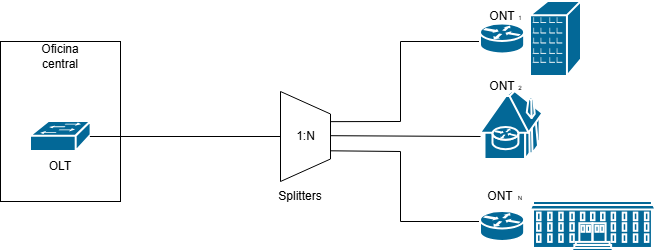
\includegraphics[width=0.8\textwidth]{Esquemas e imágenes/Esquema FTTH.png}
        \caption{Infraestructura de red FTTH}
        \label{fig:FTTH}
    \end{figure}

    \begin{itemize}
        \item OLT (Optical Line Terminal): Es el equipo activo principal ubicado en la central telefónica del proveedor de servicio. Actúa como el concentrador principal que inyecta la señal
         óptica hacia la red de distribución. La OLT es una fuente crítica en la medición de datos, ya que registra el estado de los puertos PON, las caídas masivas y las alarmas de sistemas que son capturados por el
        sistema de monitoreo de red (NOC).
        \item ODN (Optical Distribution Network): Corresponde a la red de planta externa compuesta por el cableado de fibra óptica y divisores ópticos pasivos (splitters). Es en este segmento físico continuo
        donde ocurre la mayor parte de las anomalías que el proyecto busca predecir, tales como atenuaciones por curvaturas, microcortes, empalmes defectuosos o degradaciones del material.
        \item ONT (Optical Network Terminal): Es el dispositivo activo situado en el domicilio del cliente, encargado de convertir la señal óptica en pulsos eléctricos utilizables (Ethernet, Wi-Fi). En el contexto analítico de este proyecto, las ONT actúan como
        los sensores de la última milla, proveyendo registros históricos de las potencias ópticas de recepción ($R_x$) y transmisión ($T_x$), fundamentales para evaluar una posible falla.   
    \end{itemize}


    \subsection{Acercamiento a la solución}
    \noindent
    Para dar respuesta a las limitaciones del actual modelo de mantenimiento reactivo, proponemos el diseño y desarrollo de una arquitectura analítica basada en Aprendizaje Automático. El sistema actuará como una capa
    de inteligencia operativa que complementa a la infraestructura a la red existente, procesando los registros históricos sin necesidad de intervenir físicamente la planta externa.\\\\

    \noindent
    A nivel tecnológico, la solución contempla la construcción de un pipeline de datos estructurado en fases secuenciales. Inicialmente, se implementará un proceso de extracción y limpieza de las diversas fuentes de datos crudos
    provenientes de las ONT, las OLT, los registros del sistema de monitoreo de red (NOC), entre otros. Posteriormente, mediante técnicas de Minería de datos, se extraerán patrones de comportamiento y
    fluctuaciones en la potencia óptica ($R_x$ y $T_x$) para alimentar diversos algoritmos. Esto permitirá generar un índice probabilístico de falla por segmento de red, entregando información procesable que garantice escalabilidad y flexibilidad
    en la toma de decisiones corporativas.\\\\
    
    

    \noindent
    \textbf{Elementos relevantes:}
    \begin{itemize}
        \item \textbf{Usuario:} El usuario principal directo corresponde a ingenieros de operaciones y equipo de mantenimiento de Liberty Latinamerica, quienes recibirán por notificación o correo reportes
        predictivos para gestionar personal encargado del mantenimiento preventivo. Como usuarios secundarios o beneficiarios indirectos se encuentran los clientes finales, quienes experimentarán una mejora sustancial en la QoE
        y QoS al reducir los tiempos de indisponibilidad y las incidencias técnicas.
        \item \textbf{Producto:} El producto, denominado comercialmente \textbf{PrediFibra} (Sección~\ref{sec:predifibra}), es una plataforma en la nube que procesa cada mañana la foto diaria de la red, calcula con un modelo de Machine Learning la probabilidad de que cada equipo presente una falla óptica nueva al día siguiente y genera tickets de mantenimiento preventivo priorizados en Zammad, con aviso por correo al equipo de operaciones.
        Cada alerta indica el equipo, la central, el puerto PON y, cuando la topología lo permite, el armario de distribución, lo que permite a la gerencia decidir las salidas o el despliegue de personal técnico a zona.
        \item \textbf{Valor agregado:} El contexto de aplicación se enmarca en la industria de las telecomunicaciones y la gestión de infraestructura de proveedores de servicio de internet (ISP). Se orienta hacia el nicho de mantenimiento predictivo
        inteligente, en colaboración directa con actores corporativos de Liberty Latinamerica para validar la solución en un entorno operativo real. A partir del Hito 4, la solución se plantea además como un producto comercial dirigido a operadores FTTH medianos de Latinoamérica, que se ofrece mediante un piloto pagado, una licencia y una suscripción (Sección~\ref{subsec:oferta}). 
    \end{itemize}


    \newpage
\subsection{Estado del Arte}
\noindent
El escenario actual de la gestión de infraestructuras de telecomunicaciones exhibe una transición crítica desde la reparación reactiva hacia la automatización y la inteligencia operativa. La revisión de la literatura académica reciente y de los marcos de trabajo implementados por referentes de la industria evidencia que el uso de algoritmos 
de \textbf{Machine Learning} (ML) se ha consolidado como la principal estrategia técnica para asegurar la confiabilidad en las Redes Ópticas Pasivas (PON).

\subsubsection{Confiabilidad de Red y Gestión Automatizada}
Revisiones sistemáticas sobre la confiabilidad en la industria de las telecomunicaciones coinciden en que la gestión tradicional de la infraestructura de fibra óptica es ineficiente frente a las exigencias modernas de disponibilidad 
\textbf{five-nines uptime} \cite{slr_reliability}. La investigación actual respalda la implementación de modelos de autodiagnóstico avanzados, tales como \textbf{Infinite Multivariate Categorical Mixture Models} \cite{infinite_mixture}, así como marcos automatizados de gestión de infraestructura física en redes FTTH GPON \cite{automated_gpon}, los cuales permiten a la red identificar anomalías físicas y lógicas de forma casi autónoma. Estos estudios establecen el fundamento teórico de que la telemetría pasiva contiene patrones suficientes para inferir el estado de salud de la red sin necesidad de costosas intervenciones físicas exploratorias.

\subsubsection{Tratamiento de Datos Desbalanceados mediante Modelos de Ensamble}
Uno de los mayores desafíos técnicos documentados en el entrenamiento de algoritmos para predicción de anomalías es la naturaleza asimétrica de los datos operativos (\textbf{Imbalanced Data}). En una red FTTH real, los registros históricos de funcionamiento óptimo superan abrumadoramente a los incidentes de falla. 
Para mitigar este sesgo analítico, el estado del arte propone la utilización de Modelos de Ensamble Apilados (\textbf{Stacking Ensemble ML-Based Models}) \cite{stacking_ensemble}. Estas técnicas combinan múltiples algoritmos de clasificación predictiva para aumentar la sensibilidad algorítmica frente a eventos minoritarios (las caídas de servicio), garantizando que el modelo sea capaz de aprender de los síntomas tempranos de degradación sin que la estadística general minimice la alerta.

\subsubsection{Explicabilidad Algorítmica (XAI) en Entornos Operativos}
En el ámbito corporativo, predecir una falla carece de utilidad práctica si el modelo opera como una ``caja negra''. Para abordar esto, la literatura reciente aplica técnicas de interpretabilidad o XAI (\textbf{Explainable AI}), como SHAP (\textbf{Shapley Additive exPlanations}) y 
LIME (\textbf{Local Interpretable Model-agnostic Explanations}) \cite{shap_lime}. Estas metodologías se están incorporando en el análisis de redes FTTH para cuantificar el peso matemático exacto que cada variable (por ejemplo, variaciones de potencia Rx o tasas de cortes) tiene sobre la probabilidad final de degradación, permitiendo que en el área de operaciones comprenda y confíe en la predicción.

\subsubsection{Perspectiva Industrial: Transición Analítica de la Detección a la Prevención}
Desde la perspectiva aplicada de proveedores tecnológicos y plataformas operativas, tales como Nokia \cite{nokia_predictive} y VC4 \cite{vc4_predictive}, el éxito del mantenimiento preventivo no radica exclusivamente en el algoritmo, sino en un proceso robusto de \textbf{Feature Engineering} fundamentado en el conocimiento topológico.
Las herramientas actuales correlacionan registros de estado, alarmas lógicas y desviaciones en los presupuestos de potencia (\textbf{link loss budgets}) a lo largo del tiempo. La identificación temprana de atenuaciones progresivas permite a los operadores despachar personal técnico para prevenir cortes de filamentos debido a tensiones mecánicas o microcurvaturas antes de que afecten los Acuerdos de Nivel de Servicio (SLA) de la compañía.

\subsubsection{Evaluación de Arquitecturas GPON y Aplicación Práctica en ISPs}
Además de los enfoques puramente algorítmicos, la correcta evaluación e implementación de la capa física en redes de acceso FTTH basadas en GPON es un prerrequisito fundamental. Estudios recientes detallan cómo el diseño óptimo de la red y el análisis de la atenuación pasiva condicionan el éxito de cualquier capa analítica superpuesta \cite{ftth_gpon_design}. En esta misma línea, investigaciones aplicadas directamente en los ISP confirman que el uso de \textbf{Machine Learning} en redes de fibra óptica permite detectar variaciones sutiles antes de la disrupción del 
servicio, validando la viabilidad del mantenimiento predictivo en entornos operativos \cite{isp_predictive}.

\subsubsection{Síntesis para la Arquitectura Propuesta}
Si bien la literatura actual establece bases teóricas sólidas, gran parte de las investigaciones académicas se desarrollan sobre datasets simulados o 
entornos altamente controlados. La principal diferencia y el valor agregado de esta propuesta radica en su enfoque directamente operativo e industrial.
A diferencia de los enfoques genéricos existentes, este proyecto no solo implementa técnicas para compensar el desbalanceo de clases y extraer características temporales,
sino que lo hace enfrentándose a la telemetría real y ruidosa de los sistemas de Liberty Latinamerica.\\\\

\noindent
Además, la arquitectura propuesta trasciende la mera predicción algorítmica al cerrar el ciclo de mantenimiento:
integra las probabilidades de falla calculadas con plataformas de ticketing
corporativas, traduciendo la explicabilidad algorítmica (XAI) en alertas preventivas accionables,
resolviendo así la problemática del mantenimiento reactivo en un operador a gran escala con una solución técnica lista para su evaluación en terreno. 

 

    \section{Requisitos del Sistema:}  

        \subsection{\textbf{Requerimientos Funcionales:}}
                    \begin{itemize}
                        \item \textbf{RF1.} Extracción de datos: El sistema debe ser capaz de cargar y leer múltiples archivos de datos estructurados.
                        \item \textbf{RF2.} Limpieza y preprocesamiento: El sistema debe ejecutar ciclos períodicos para limpiar los archivos, específicamente, manejar valores nulos, eliminar datos duplicados, corregir formatos de datos (Por ejemplo, transformar fechas a "dd-MM-yyyy"), filtrar ruido en las mediciones y datos inconsistentes.
                        \item \textbf{RF3.} Feature Engineering: El sistema debe generar nuevas variables calculadas a partir de datos ya procesados (por ejemplo, calcular potencia óptica en diferentes periodos según la medición diaria).
                        \item \textbf{RF4.} Visualización de distribución: Visualizar la distribución de datos mediante gráficos y obtener valores estadísticos para la toma de decisión en la elección de los algoritmos a utilizar.
                        \item \textbf{RF5.} Entrenamiento y validación: El sistema debe permitir entrenar algoritmos de aprendizaje automático utilizando el conjunto de datos históricos previamente procesados y validados según su rendimiento mediante técnicas como \textbf{Cross-validation}.
                        \item \textbf{RF6.} Generación de predicciones: El sistema debe evaluar los nuevos datos ingresados y emitir una probabilidad de degradación o falla por algún equipo (ONT/OLT) en algún segmento de red específico.
                        \item \textbf{RF7.} Evaluación de métricas: El sistema deberá calcular y mostrar métricas de rendimiento del modelo (Por ejemplo, Precisión, Recall, F1-Score, Matriz de confusión, entre otros). 
                        \item \textbf{RF8.} Generación de tickets: El sistema debe comunicarse mediante una API REST con la plataforma Zammad para crear incidencias de mantenimiento de forma automática.
                        \item \textbf{RF9.} Notificación al usuario: El sistema debe enviar alertas estructuradas por correo electrónico al personal técnico detallando el segmento de red en riesgo.
                    \end{itemize}
        \subsection{\textbf{Requerimientos de Interfaces:}}
                    \begin{itemize}
                        \item Interfaz de datos: El sistema requiere de una lectura de archivos locales o en un servicio de nube que soporte los formatos \textbf{.csv}, \textbf{.xlsx} y \textbf{.xls}.
                        \item Interfaz de Salida: El sistema deberá exportar las predicciones generadas a un formato estandarizado (por ejemplo, un archivo \textbf{.csv} con el identificador del equipo y su probabilidad de falla) para que pueda ser interpretado por la gerencia.
                        \item Interfaz de Usuario: Visualizar los resultados mediante un reporte notificado por correo electrónico.
                    \end{itemize}
        \subsection{\textbf{Requerimientos de Ambiente:}}
                    \begin{itemize}
                        \item \textbf{Requerimientos de Software:} 
                        \begin{enumerate}
                            \item Python versión 3.8 o superior.
                            \item Librerías de procesamiento y modelado de datos: Pandas, numpy, matplotlib, Gym, Sckit-learn, XGBoost, pytorch, Tensorflow, dependiendo de las necesidades y arquitectura a escoger.
                            \item Sistema operativo compatible con el entorno de desarrollo (Windows/Linux).
                        \end{enumerate}
                        \item \textbf{Requerimientos de Hardware:}
                        \begin{enumerate}
                            \item \textbf{Memoria RAM:} Se recomienda tener un mínimo de 16 GB o 32 GB de RAM para el procesamiento de datos y unificación de datasets, evitando así, un cuello de botella en la limpieza de varios excels.
                            \item \textbf{Procesamiento (CPU/GPU):} La elección dependerá de la arquitectura de entrenamiento a utilizar. Procesador Multi-núcleo para paralelizar el entrenamiento o tareas de secuencias complejas de pocos núcleos, especialmente útil en técnicas de aprendizaje reforzado de algoritmos como Actor-Crítico (A2C). El uso de la GPU será de gran ventaja en el procesamiento de múltiples hilos ejecutando aritmética básica, siendo especialmente útil en el entrenamiento de redes neuronales profundas. 
                        \end{enumerate}
                        \item \textbf{Entorno de ejecución:} Será necesario requerir un entorno de ejecución en la nube dado un volumen de datos pesado. Por lo que se recomienda contar con una licencia de Google colab (existen otras opciones) que permita seleccionar un hardware con mayor capacidad de cómputo. 
                    \end{itemize}
                


    \section{Planificación del Proyecto}
    \subsection{Objetivo General}
    \noindent
    Desarrollar y validar el pipeline y modelo predictivo basado en algoritmos de aprendizaje automático capaz de anticipar degradaciones físicas en la infraestructura FTTH de Liberty Latinamerica, proporcionando estimaciones probabilísticas
    de falla para optimizar el mantenimiento preventivo y reducir los tiempos de indisponibilidad del servicio, mejorando la experiencia del usuario final y la eficiencia operativa de la compañía.

    \subsection{Objetivos específicos}
    \begin{enumerate}
        \item \textbf{OE1:} Analizar el estado del arte y seleccionar los algoritmos del Aprendizaje automático con mejor desempeño para el procesamiento de datos de redes ópticas y predicción de fallas.
        \item \textbf{OE2:} Desarrollar el pipeline de datos y entrenar los modelos predictivos utilizando los registros históricos de todos los dispositivos y sistema de monitoreo de red.
        \item \textbf{OE3:} Medir y evaluar las métricas de precisión de los modelos entrenados utilizando datasets validados contra el comportamiento histórico de la red real, asegurando su viabilidad para aplicarse en operaciones en terreno.
        \item \textbf{OE4:} Implementar un sistema de notificaciones destinado a los usuarios objetivo que muestre un reporte de incidencia de posibles fallas y estado general de la red.
    \end{enumerate}

    \subsection{Actividades y Milestones}
    \noindent
    

    \subsubsection{Módulo 1: Identificación de técnicas que permitan realizar predicciones}


        \begin{table}[H]
            \centering
            \renewcommand{\arraystretch}{1.5}
            \begin{tabular}{|p{5cm}|p{3cm}|p{2cm}|p{2cm}|p{2cm}|}
            \hline
            \textbf{Actividad} & \textbf{Responsable} & \textbf{Fecha de comienzo} & \textbf{Fecha de término} & \textbf{\% de avance} \\ \hline
            \textbf{OE1: Identificación de técnicas que permitan realizar predicciones} & Gabriel Zapata, Yu Zhou & 22-04-2026 & 20-05-2026 & 100\% \\ \hline
            A1.1: Revisión del estado del arte & Gabriel Zapata, Yu Zhou & 22-04-2026 & 17-05-2026 & 100\% \\ \hline
            T1.1.1: Elaboración de una estrategia de búsqueda & Gabriel Zapata & 22-04-2026 & 11-05-2026 & 100\% \\ \hline
            T1.1.2: Búsqueda de literatura sobre mantenimiento predictivo en redes FTTH & Gabriel Zapata, Yu Zhou & 22-04-2026 & 17-05-2026 & 100\% \\ \hline
            A1.2: Entender la naturaleza de los datos actuales de la FTTH & Gabriel Zapata, Yu Zhou & 22-04-2026 & 20-05-2026 & 100\% \\ \hline
            T1.2.1: ONT & Gabriel Zapata & 22-04-2026 & 20-05-2026 & 100\% \\ \hline
            T1.2.2: PON & Yu Zhou & 22-04-2026 & 20-05-2026 & 100\% \\ \hline
            \end{tabular}
            \caption{Planificación OE1}
            \label{tab:planificacion_avance}
        \end{table}

    \subsubsection{Módulo 2: Entrenar modelos predictivos}



    \begin{table}[H]
            \centering
            \renewcommand{\arraystretch}{1.5}
            \begin{tabular}{|p{5cm}|p{3cm}|p{2cm}|p{2cm}|p{2cm}|}
            \hline
            \textbf{Actividad} & \textbf{Responsable} & \textbf{Fecha de comienzo} & \textbf{Fecha de término} & \textbf{\% de avance} \\ \hline
            \textbf{OE2: Entrenar modelos predictivos} & Gabriel Zapata, Yu Zhou & 20-05-2026 & 20-07-2026 & 100\% \\ \hline
            A2.1: Preparación del pipeline de datos & Gabriel Zapata, Yu Zhou & 20-05-2026 & 15-06-2026 & 100\% \\ \hline
            T2.1.1: Limpieza, normalización y manejo de valores nulos & Gabriel Zapata, Yu Zhou & 20-05-2026 & 25-05-2026 & 100\% \\ \hline
            T2.1.2: Reducción de dimensionalidad & Gabriel Zapata & 25-05-2026 & 29-05-2026 & 100\% \\ \hline
            T2.1.3: Feature engineering & Gabriel Zapata & 29-05-2026 & 04-06-2026 & 100\% \\ \hline
            A2.2: Entrenamiento de modelos candidatos & Yu Zhou & 04-06-2026 & 20-07-2026 & 100\% \\ \hline
            T2.2.1: Optimización de hiperparámetros & Yu Zhou & 04-06-2026 & 20-07-2026 & 100\% \\ \hline
            \end{tabular}
            \caption{Planificación OE2}
            \label{tab:planificacion_avance_oe2}
    \end{table}




    \subsubsection{Módulo 3: Medir los resultados de los modelos en un ambiente real}


    \begin{table}[H]
            \centering
            \renewcommand{\arraystretch}{1.5}
            \begin{tabular}{|p{5cm}|p{3cm}|p{2cm}|p{2cm}|p{2cm}|}
            \hline
            \textbf{Actividad} & \textbf{Responsable} & \textbf{Fecha de comienzo} & \textbf{Fecha de término} & \textbf{\% de avance} \\ \hline
            \textbf{OE3: Medir los resultados de los modelos en un ambiente real} & Gabriel Zapata, Yu Zhou & 10-07-2026 & 20-08-2026 & 88\% \\ \hline
            A3.1: Evaluación estadística & Gabriel Zapata & 10-07-2026 & 24-07-2026 & 100\% \\ \hline
            T3.1.1: Elaboración de matriz de confusión a partir de resultados actuales & Gabriel Zapata & 10-07-2026 & 17-07-2026 & 100\% \\ \hline
            T3.1.2: Cálculo de Precision, Recall y F1 & Gabriel Zapata & 17-07-2026 & 24-07-2026 & 100\% \\ \hline
            A3.2: Evaluación económica & Yu Zhou & 24-07-2026 & 20-08-2026 & 75\% \\ \hline
            T3.2.1: Cálculo de CapEx y OpEx & Yu Zhou & 24-07-2026 & 17-08-2026 & 100\% \\ \hline
            T3.2.2: Estudio de factibilidad del modelo & Yu Zhou & 17-08-2026 & 20-08-2026 & 50\% \\ \hline
            \end{tabular}
            \caption{Planificación OE3}
            \label{tab:planificacion_avance_oe3}
    \end{table}



    \subsubsection{Módulo 4: Desarrollo de sistema de notificaciones}
    \begin{table}[H]
            \centering
            \renewcommand{\arraystretch}{1.5}
            \begin{tabular}{|p{5cm}|p{3cm}|p{2cm}|p{2cm}|p{2cm}|}
            \hline
            \textbf{Actividad} & \textbf{Responsable} & \textbf{Fecha de comienzo} & \textbf{Fecha de término} & \textbf{\% de avance} \\ \hline
            \textbf{OE4: Desarrollo de sistema de notificaciones} & Gabriel Zapata, Yu Zhou & 20-08-2026 & 04-09-2026 & 94\% \\ \hline
            A4.1: Definición del flujo del sistema & Yu Zhou & 20-08-2026 & 22-08-2026 & 100\% \\ \hline
            T4.1.1: Elección de formato de entradas y salidas & Yu Zhou & 20-08-2026 & 21-08-2026 & 100\% \\ \hline
            T4.1.2: Elección de plataforma para la notificación & Yu Zhou & 21-08-2026 & 22-08-2026 & 100\% \\ \hline
            A4.2: Automatización del proceso & Gabriel Zapata, Yu Zhou & 22-08-2026 & 04-09-2026 & 88\% \\ \hline
            T4.2.1: Selección de las herramientas de automatización & Gabriel Zapata, Yu Zhou & 22-08-2026 & 27-08-2026 & 100\% \\ \hline
            T4.2.2: Implementación y prueba del sistema & Gabriel Zapata, Yu Zhou & 27-08-2026 & 04-09-2026 & 75\% \\ \hline
            \end{tabular}
            \caption{Planificación OE4}
            \label{tab:planificacion_avance_oe4}
    \end{table}

    \noindent
    Al cierre del Hito 4 quedan dos tareas parciales. En T3.2.2 (50\,\%) se cuenta con el costo de operación y con la comparación entre proveedores de nube (Sección~\ref{subsec:costos}), pero falta contrastar ese costo con el ahorro que genera cada falla anticipada, lo que requiere conocer el costo de una visita correctiva. En T4.2.2 (75\,\%) la cadena se probó de punta a punta con la lista de riesgo del 29 de septiembre, con tickets reales en Zammad y su correo; falta automatizar la recepción diaria de los datos, programar la corrida diaria y cargar el modelo final en la plataforma.


    \begin{figure}[H]
            \centering
            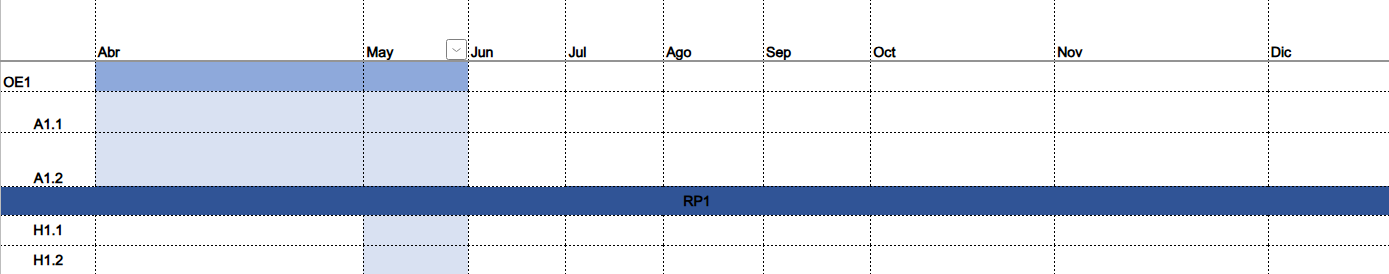
\includegraphics[width=1\textwidth]{Esquemas e imágenes/GANTT1.png}
            \caption{Gantt OE1}
    \end{figure}
    \begin{figure}[H]
            \centering
            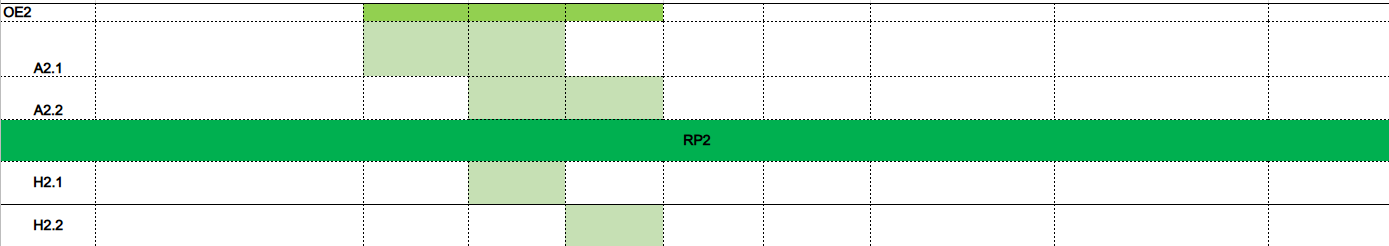
\includegraphics[width=1\textwidth]{Esquemas e imágenes/GANTT2.png}
            \caption{Gantt OE2}
    \end{figure}
    \begin{figure}[H]
            \centering
            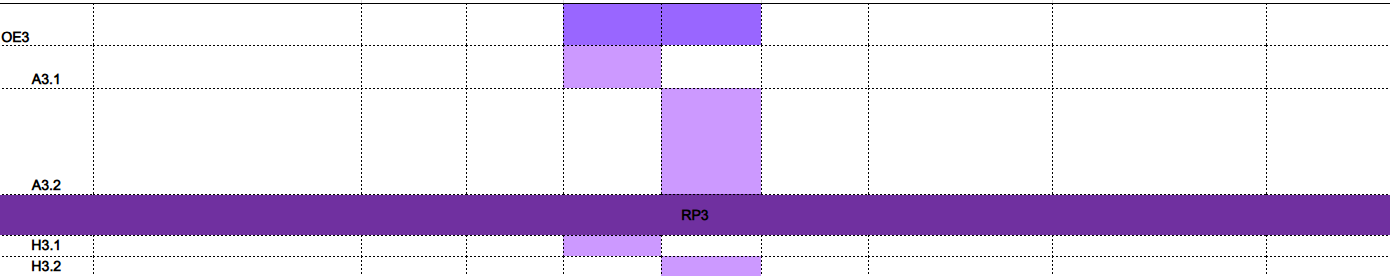
\includegraphics[width=1\textwidth]{Esquemas e imágenes/GANTT3.png}
            \caption{Gantt OE3}
    \end{figure}
    \begin{figure}[H]
            \centering
            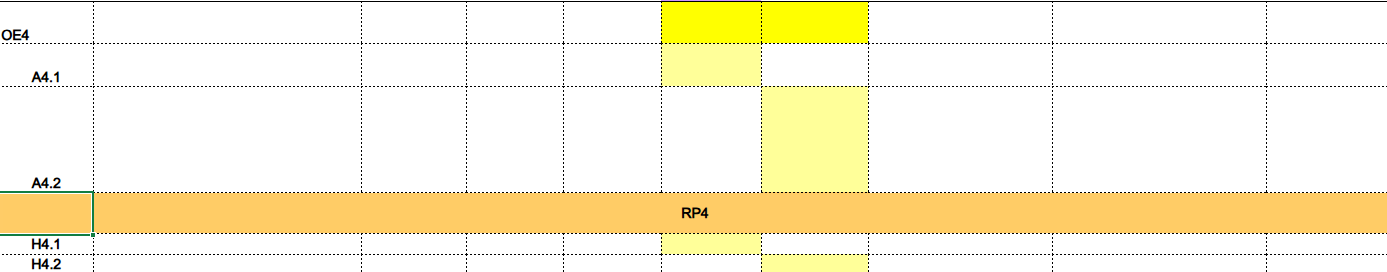
\includegraphics[width=1\textwidth]{Esquemas e imágenes/GANTT4.png}
            \caption{Gantt OE4}
    \end{figure}





\newpage
  \section{Arquitectura del Sistema:}


    \subsection*{\textbf{Diagrama de Contexto}}
    \noindent
    El siguiente diagrama muestra la interacción de los distintos dispositivos con el sistema. Se observa la entrada que recibe el modelo predictivo (Desde las ONT, OLT y NOC) y la 
    salida, en donde realiza una llamada a la API de Zammad para emitir el reporte al equipo de LLA.

    \begin{figure}[H]
            \centering
            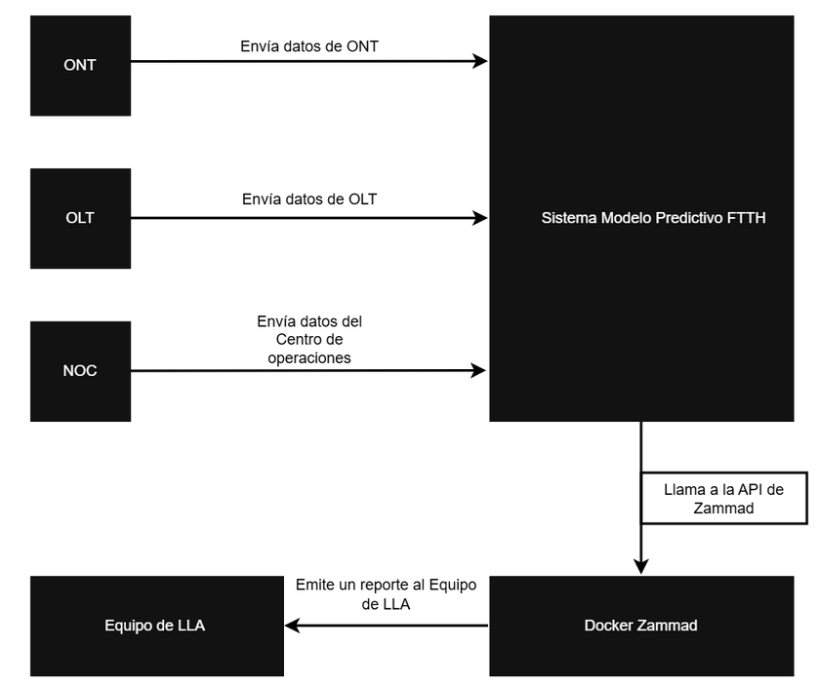
\includegraphics[width=0.6\textwidth]{Esquemas e imágenes/Diagrama Contexto.png}
            \caption{Diagrama de contexto}

    \end{figure}


    \subsection{\textbf{Diagrama de Arquitectura:}} 
    \noindent
    La figura \ref{MODELO ML} resume la arquitectura de alto nivel del modelo predictivo destinado para la posible detección de degradaciones en la red FTTH. La descripción de cada bloque se especifica en el cuadro 5.

                    \begin{figure}[H]
                        \centering
                        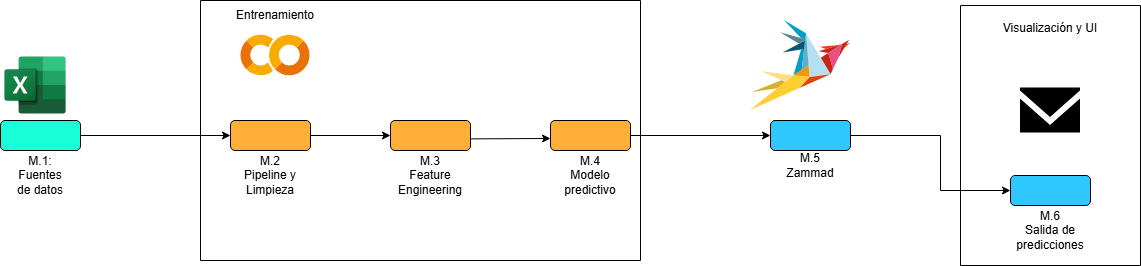
\includegraphics[width=0.8\textwidth]{Esquemas e imágenes/Fases de arquitectura ML.png}
                        \caption{Arquitectura del sistema}
                        \label{MODELO ML}
                    \end{figure}
    \subsection{\textbf{Descripción General de Módulos:}}
                
                    \begin{table}[H]
                        \centering
                        \begin{tabularx}{\textwidth}{|p{3.5cm}|X|p{2cm}|}
                            \hline
                            \rowcolor{black} 
                            \textcolor{white}{Módulos} & \textcolor{white}{Propósito} & \textcolor{white}{Sección}  \\ \hline
                            
                            \textbf{M.1: Fuentes de datos} & El módulo extrae la información de manera estática. Esto incluye: mediciones de potencia óptica (Rx/Tx) provenientes de las ONT, registros de estado de los puertos PON, alarmas, entre otros. & 5.1 \\ \hline
                            \textbf{M.2: Pipeline y Limpieza} & El módulo realiza la consolidación de las distintas fuentes mediante identificadores en común (número serial del dispositivo/ID del cliente y el puerto lógico de la OLT). Además, se realiza una limpieza de datos cuyas acciones incluyen: manejo de valores nulos, registros duplicados y estandarización de formatos. & 5.2 \\ \hline
                            \textbf{M.3: Feature Engineering} & Crea nuevas variables matemáticas a partir de los datos históricos para ayudar al modelo a encontrar patrones de degradación. & 5.3 \\ \hline
                            \textbf{M.4: Modelo predictivo} & Los algoritmos de machine learning (Por ejemplo, Random Forest, XGBoost, Redes neuronales profundas, aprendizaje reforzado). Durante la fase de desarrollo, este componente aprende los patrones de falla. En producción, toma los datos nuevos y calcula la probabilidad de degradación. & 5.4 \\ \hline
                            \textbf{M.5: Integración de Ticketing Zammad} & Actúa como puente automatizado. Recibe las predicciones críticas del modelo e invoca la API de Zammad para registrar formalmente una alerta operativa de mantenimiento. & 5.5 \\ \hline
                            \textbf{M.6: Visualización y UI (Correo electrónico)} & Interfaz final que traduce el ticket generado en un reporte ejecutivo y lo notifica pasivamente al personal técnico mediante correo electrónico. & 5.6 \\ \hline
                        \end{tabularx}
                        \caption{Descripción de cada componente}
                        \label{Tabla MODULO}
                    \end{table}


                
    \subsection{\textbf{Matriz de Requisitos Funcionales y Componentes:}}
                
                    \begin{table}[H]
                        \centering
                        \begin{tabularx}{\textwidth}{|X|p{1cm}|p{1cm}|p{1cm}|p{1cm}|p{1cm}|p{1cm}|}
                            \hline
                            \rowcolor{black} 
                            \textcolor{white}{Requerimiento} & \textcolor{white}{M.1} & \textcolor{white}{M.2} & \textcolor{white}{M.3} & \textcolor{white}{M.4} & \textcolor{white}{M.5} & \textcolor{white}{M.6}  \\ \hline
                            
                            \textbf{RF1} & X & & & & & \\ \hline
                            \textbf{RF2} & & X & & & & \\ \hline
                            \textbf{RF3} & & & X & & & \\ \hline
                            \textbf{RF4} & & & X & X & &  \\ \hline
                            \textbf{RF5} & & & & X & & \\ \hline
                            \textbf{RF6} & & & & X & & \\ \hline
                            \textbf{RF7} & & & & X &  & \\ \hline
                            \textbf{RF8} & & & &  & X & \\ \hline
                            \textbf{RF9} & & & &  &  & X \\ \hline
                        \end{tabularx}
                    \end{table}
    
    \section{Diseño de Módulos del Sistema:}
    \label{sec:modulos}
    \subsection{Fuentes de datos:}

    \begin{itemize}
        \item \textbf{Propósito:} El módulo es el responsable de extraer y recopilar la información cruda de la infraestructura. Este módulo se encarga de reunir por telemetría los datos asociados
        a todos los dispositivos de la red de forma estática y dinámica, incluyendo mediciones de Potencia ($R_x/T_x$), registros de alarma y estado de los puertos PON, entre otros. 

        \item \textbf{Alcance:} Este es el módulo inicial del sistema, encargado de obtener el insumo principal de datos para alimentar el pipeline de procesamiento. 
        
        \item \textbf{Dependencias:}
        
        \begin{itemize}
            \item \textbf{Equipos de red:} Este módulo requiere acceso a los registros exportados provenientes de los dispositivos de red.
        \end{itemize}

        \item \textbf{Supuestos:} Se asume que los sistemas de registro de la empresa no presentarán interrupciones significativas y que la data histórica abarca un periodo suficiente para encontrar patrones.
        \item \textbf{Restricciones:} El módulo debe ser capaz de manejar grandes volúmenes sin consumir recursos computacionales excesivos.
        \item \textbf{Estructura General:}
        \begin{itemize}
            \item \textbf{Entradas:} Archivos estáticos en formato Excel con registros de la red FTTH.
            \item \textbf{Ejecución:} Leer y cargar en memoria los archivos provenientes de la medición de los dispositivos(ONT y OLT) y NOC.
            \item \textbf{Salidas:} Enviar las estructuras de datos crudos (Dataframes) al módulo de pipeline y limpieza.
        \end{itemize}
    \end{itemize}


    \subsection{Pipeline y limpieza:}

    \begin{itemize}
        \item \textbf{Propósito:} Este módulo es el responsable de consolidar las distintas fuentes de información mediante el cruce de identificadores comunes (número serial del dispositivo/ID del cliente y el puerto lógico de la OLT). Además,
         modifica y limpia los datos manejando valores nulos, eliminando duplicados y estandarizando su formato.
        \item \textbf{Alcance:} Actúa como el intermediario fundamental entre los datos en bruto y el procesamiento matemático avanzado.
        \item \textbf{Dependencias:} Depende directamente de la información cruda obtenida por el módulo anterior.
        \item \textbf{Supuestos:} Se asume que el formato de las columnas exportadas desde los sistemas corporativos se mantendrá constante en el tiempo.
        \item \textbf{Restricciones:}
        \begin{itemize}
            \item Las técnicas de limpieza y filtrado de valores nulos no deben alterar significativamente la distribución real de las métricas ópticas.
        \end{itemize}
        \item \textbf{Estructura General:} 
        \begin{itemize}
            \item \textbf{Entradas:} Datos crudos obtenidos del módulo anterior.
            \item \textbf{Ejecución:} 
            \begin{itemize}
                \item Unificar tablas de llaves primarias (identificadores en común).
                \item Filtrar información corrupta, duplicados o datos inconsistentes.
                \item Estandarizar los tipos de datos y formatos.
            \end{itemize}
            \item \textbf{Salidas:} Enviar un conjunto de datos consolidado y limpio al módulo de Feature Engineering.
        \end{itemize}
    \end{itemize}


    \subsection{Feature Engineering}
    \begin{itemize}
        \item \textbf{Propósito:} El módulo es el encargado de crear nuevas variables matemáticas predictivas a partir de los datos históricos. Su objetivo es transformar las métricas aisladas
        en indicadores de tendencia y variación temporal que faciliten al algoritmo encontrar los patrones de degradación física. Además, implementa técnicas de reducción de dimensionalidad para facilitar y optimizar la carga computacional del entrenamiento del
        modelo en el siguiente módulo.
        \item \textbf{Alcance:} Es el paso final de preparación de datos antes del entrenamiento del modelo predictivo.
        \item \textbf{Dependencias:} Requiere el dataset unificado y estandarizado proveniente del módulo de Pipeline y Limpieza.
        \item \textbf{Supuestos:} Se asume que la degradación física en la planta externa tiene un comportamiento temporal progresivo que puede ser capturado mediante el cálculo de tendencias.
        \item \textbf{Restricciones:} La complejidad en el cálculo de las nuevas características (como medias móviles) podría requerir tiempos de ejecución elevados, dependiendo del tamaño del dataset.
        \item \textbf{Estructura General:}
        \begin{itemize}
            \item \textbf{Entradas:} Dataset histórico consolidado y limpio.
            \item \textbf{Ejecución:}
             \begin{itemize}
                \item \textbf{Creación de variables temporales y de agregación:} Se calcularán métricas con sentido físico, tales como: Medias móviles de Potencia de Recepción $R_x$, en ventanas de 7, 14 y 30 días; diferencia temporal de potencia de transmisión $T_x$ respecto a la mediana histórica
                 del puerto; y el conteo acumulado de fluctuaciones o alarmas PON en las últimas 24 y 48 horas.
                \item \textbf{Reducción de dimensionalidad:} Aplicación de técnicas estadísticas PCA, o análisis de correlación Pearson para eliminar variables colineales que no aportan una varianza
                explicativa al estado de la red.
            \end{itemize}
        \end{itemize}
        \item \textbf{Salidas:} Se obtiene un Dataframe procesado, enriquecido con características temporales y optimizado dimensionalmente, listo para el entrenamiento. 
    \end{itemize}


    \subsection{Modelo predictivo}
    \label{subsec:modelo}
    \begin{itemize}
        \item \textbf{Propósito:} Este módulo es el encargado de aplicar y entrenar el modelo mediante un conjunto de algoritmos de Machine learning (como Random Forest, XGBoost, regresiones, Kernel machines, aprendizaje reforzado, entre otros) para evaluar y seleccionar el mejor de ellos para predecir
        predecir la probabilidad de degradación en los enlaces FTTH.

        \item \textbf{Alcance:} Abarca desde el consumo del dataset procesado y enriquecido hasta la exportación del modelo matemático ajustado para inferencias futuras.
        \item \textbf{Dependencias:}
        \begin{itemize}
            \item Depende de la calidad y representatividad de las características extraídas en el módulo de Feature Engineering.
        \end{itemize}
        \item \textbf{Supuestos:} Se asume que el dataset histórico contiene suficientes registros etiquetados implícitamente como una falla frente a un abrumador volumen de comportamiento normal.
        \item \textbf{Restricciones:} El entrenamiento debe mitigar el overfitting provocado por el fuerte desbalance de clases propio de las redes operativas.
        \item \textbf{Estructura General:}
        \begin{itemize}
            \item \textbf{Entradas:} Dataframe limpio con las variables enriquecidas.
            \item \textbf{Ejecución:}
            \begin{itemize}
                \item Se aplicarán técnicas de remuestreo como SMOTE o ajuste de pesos en la función de pérdida para manejar el desbalance de clases.
                \item Metodología de selección: Se entrenarán modelos candidatos de distintas naturaleza.
                \item Debido al impacto operativo de falsos negativos (fallas no detectadas), el modelo final no se seleccionará por su exactitud, sino aquel que maximice la métrica 
                F1-Score y la sensibilidad del área bajo la curva de precisión ($PR-AUC$) durante la validación cruzada.
            \end{itemize}
            \item \textbf{Salidas:} Archivo serializado que contiene el modelo óptimo entrenado y listo para recibir nuevos datos y emitir predicciones probabilísticas.
        \end{itemize}
    \end{itemize}

    \subsection{Integración con Plataforma de Ticketing (Zammad)}
    \label{subsec:zammad}
    \begin{itemize}
        \item \textbf{Propósito:} Este módulo actúa como el puente de comunicación automatizado entre el Modelo Predictivo y la capa de operaciones. Su función es recibir los hallazgos de degradación del modelo e invocar la API de Zammad para registrar formalmente una alerta de mantenimiento preventivo.
        \item \textbf{Alcance:} Comprende la recepción de los datos del modelo, la estructuración del payload y la comunicación de red con el sistema de Helpdesk.
        \item \textbf{Dependencia:} Depende directamente de las predicciones de probabilidad emitidas por el Módulo 5.4 y de la disponibilidad de la API REST de Zammad.
        \item \textbf{Supuestos:} Se asume que Zammad cuenta con los endpoints configurados para recibir solicitudes automatizadas (peticiones HTTP) sin requerir autenticación manual en cada evento.
        \item \textbf{Restricciones:} El módulo debe contar con una lógica de control para evitar la duplicación de tickets operativos si el modelo detecta repetidamente la misma falla en ventanas de tiempo muy cortas.
        \item \textbf{Estructura General:} 
        \begin{itemize}
            \item \textbf{Entradas:} Identificadores del equipo afectado (Ej. OLT, puerto PON, ONT) y la probabilidad de falla calculada por el modelo predictivo.
            \item \textbf{Ejecución: } 
            \begin{itemize}
                \item Evaluación de la probabilidad frente al umbral crítico predefinido.
                \item Construcción del payload en formato JSON con los datos del equipo y la severidad del riesgo (Probabilidad de falla).
                \item Ejecución de la llamada a la API de Zammad para la apertura del ticket.
            \end{itemize} 
            \item \textbf{Salidas:} Un ticket de incidencia generado exitosamente en la plataforma de gestión de la compañía.
        \end{itemize}
    \end{itemize}

    \subsection{Salida de predicción y Notificación}
    \begin{itemize}
        \item \textbf{Propósito:} Constituye la interfaz directa con el usuario final, encargada de notificar al personal técnico o administrativo de forma pasiva y sin generar fricción cognitiva.

        \item \textbf{Alcance:} Abarca el despliegue del reporte final mediante el envío de un correo electrónico automatizado con los detalles esenciales de la anomalía.
        \item \textbf{Dependencias:} Depende de la correcta generación del ticket en el módulo 5.5 (Zammad), el cual dispara la notificación.
        \item \textbf{Supuestos:} Se asume que el usuario final del área de operaciones tiene acceso regular y conectividad a su bandeja de correo corporativo para recibir y revisar la alerta de manera oportuna.
        \item \textbf{Restricciones:} El formato visual del reporte (correo electrónico) debe ser estrictamente en formato HTML ligero sin requerir la carga de imágenes pesadas o complementos externos, garantizando su correcta y rápida visualización en dispositivos móviles en terreno.
        \item \textbf{Estructura General:} 
        \begin{itemize}
            \item \textbf{Entradas:} Confirmación de creación del ticket en Zammad y metadatos asociados (Ubicación física/lógica).
            \item \textbf{Ejecución:}
            \begin{itemize}
                \item Formateo de la información en una plantilla de correo electrónico estandarizada, priorizando la jerarquía visual de la información crítica.
                \item Inclusión de un resumen que contenga la ubicación exacta del segmento de red degradado, el equipo específico y la probabilidad de falla inminente.
            \end{itemize}
            \item \textbf{Salidas:} Correo electrónico de alerta despachado y entregado en la bandeja de entrada del usuario objetivo.
        \end{itemize}
    \end{itemize}
                

\section{Marco General}
\noindent
Recapitulando, el proyecto consiste en el desarrollo de un modelo predictivo
de Machine Learning para la detección temprana de anomalías en la red FTTH de Liberty Latinamerica, complementando con
un sistema de notificaciones automatizados que traduce las predicciones en alertas accionables
para el personal técnico. En el Hito 3 se consolidó el pipeline desde la extracción de fuentes crudas
hasta un dataset unificado listo para el entrenamiento, y se definió y validó la variable objetivo del modelo. En el Hito 4 se eligió y evaluó el modelo, se conectó la plataforma de punta a punta en Azure y se formuló la propuesta comercial PrediFibra (Sección~\ref{sec:predifibra}).

\subsection{Hitos Principales del Proyecto}

\begin{itemize}
    \item \textbf{Hito 1 (definición):} Levantamiento del problema, definición de alcances, requisitos funcionales y de ambiente, revisión del estado del arte
    y arquitectura conceptual de la solución.
    \item \textbf{Hito 2 (diseño detallado):} especificación de los seis módulos del sistema (M.1 Fuentes de datos, M.2 Pipeline y Limpieza, M.3 Feature Engineering, M.4 Modelo Predictivo, M.5 Integración Zammad, M.6 Visualización y UI), diagramas de contexto y arquitectura,
    matriz de requerimientos funcionales y diseño de la interfaz de notificación.
    \item \textbf{Hito 3 (Prototipo):} Implementación funcional de los módulos M.1, M.2 y M.3. Se consolidó 8 de las 13 fuentes de datos en un dataset unificado de 999.766 registros a nivel de ONT por día. Se definió
    la variable objetivo (falla\_optica) con criterio técnico y se validó contra una fuente de monitoreo independiente; se ejecutaron tres iteraciones, evaluados cuantitativamente mediante entrenamientos exploratorios
    que triplicaron la capacidad predictiva medida respecto a la línea base. Adicionalmente, se implementó la integración con la plataforma Zammad (M.5), pendiente de conexión con la salida del modelo. La selección
    del modelo definitivo aún no forma parte del alcance de este hito.
    
    \item \textbf{Hito 4 (Prototipo comercial):} Ampliación de los datos a 61 días (14.442.061 equipo-días de 279.964 equipos), procesados con DuckDB y Parquet. La tarea se redefinió como la anticipación de fallas ópticas nuevas para el día siguiente; se eligieron 25 de 47 variables candidatas y se compararon cuatro modelos optimizados con Optuna, eligiéndose LightGBM con dos semanas de validación.
    En una semana de prueba nunca vista, el modelo ordenó los equipos 17,5 veces mejor que el azar y, con 25 alertas diarias, 1 de cada 9 correspondió a una falla nueva al día siguiente. Se conectó la plataforma de punta a punta en Azure (modelo, Zammad y correo) y se formuló la oferta comercial PrediFibra con sus costos de operación (Sección~\ref{sec:predifibra}).

    \item \textbf{Siguiente etapa (planificada):} Piloto pagado de tres meses con evaluación semanal, registro de la causa de cierre de cada ticket, incorporación de los motivos SHAP al ticket, reentrenamiento con más historia y propuesta de detección sobre mediciones horarias (Sección~\ref{subsec:hoja_ruta}).
\end{itemize}


\subsection{Revisión de Requerimientos}

\begin{table}[H]
\centering
\small 
\renewcommand{\arraystretch}{1.3}
\begin{tabular}{|p{1.1cm}|p{2.9cm}|p{1.9cm}|p{7.2cm}|}
\hline
\textbf{RF} & \textbf{Descripción} & \textbf{Estado H4} & \textbf{Evidencia / Comentarios} \\
\hline
RF1 & Extracción de datos & Cumplido & En el Hito 4, siete fuentes leídas con DuckDB: cuatro diarias de 61 días en Parquet (ONT, portstats, puertos PON y alarmas NCE) y tres fijas en .csv (circuitos, infraestructura y soporte). El Hito 3 cargó 13 archivos de mayo. \\
\hline
RF2 & Limpieza y preprocesamiento & Cumplido & Corrección de formatos de fecha, tipificación de identificadores, tratamiento de valores centinela y deduplicación por clave primaria con desempates fijos (resultados reproducibles). \\
\hline
RF3 & Feature Engineering & Cumplido & 47 variables candidatas (márgenes ITU-T, tendencias de 7 días, historial de fallas, vecinos del puerto PON y de la OLT, NCE del día anterior); se conservaron 25 (Sección~\ref{subsec:revision_diseno}). \\
\hline
RF4 & Visualización de distribución & Cumplido & Análisis exploratorio de distribuciones, cobertura por fuente, tasa de eventos por segmento y señales previas a una falla nueva. \\
\hline
RF5 & Entrenamiento y validación & Cumplido & Cuatro modelos optimizados con Optuna y validados en el tiempo con dos semanas; se eligió LightGBM (Cuadro~\ref{tab:modelos}). \\
\hline
RF6 & Generación de predicciones & Cumplido & Probabilidad de falla óptica nueva al día siguiente para cada equipo; punto de operación de 25 alertas diarias. \\
\hline
RF7 & Evaluación de métricas & Cumplido & Matriz de confusión, precisión, recall, F1, PR-AUC y ROC-AUC en la semana de prueba (Cuadro~\ref{tab:confusion}). \\
\hline
RF8 & Generación de tickets & Cumplido & Tickets en Zammad vía API REST desde la lista de riesgo, con un máximo de un ticket abierto por segmento. \\
\hline
RF9 & Notificación al usuario & Cumplido & Correo HTML desde Zammad con alertas reales del modelo (FTTH\#63002 a FTTH\#63004). \\
\hline
\end{tabular}
\caption{Estado de cobertura de los Requisitos Funcionales al Hito 4}
\label{tab:cobertura-rf}
\end{table}

\subsubsection*{Requisitos No Funcionales y de Ambiente}

\begin{itemize}
    \item \textbf{Formatos de entrada (.csv, .xlsx, .xls):} cumplido. El pipeline procesa ambos formatos sin intervención manual.

    \item \textbf{Manejo de volumen:} cumplido. Los 14.442.061 equipo-días del Hito 4 se procesan con DuckDB y archivos Parquet en el equipo local, sin requerir infraestructura de Big Data, lo que valida el supuesto S3 declarado en el Hito 2. El entrenamiento usa una muestra con todas las fallas y el 5\,\% de los casos sin falla, ponderados para conservar la proporción real.
 
    \item \textbf{Confidencialidad de la información (R2):} cumplido. El trabajo se realiza sobre identificadores técnicos de equipos y cuentas, sin exposición de datos personales de clientes.
 
    \item \textbf{Preservación de la distribución real en la limpieza:} cumplido. Las técnicas de tratamiento de valores faltantes se aplicaron distinguiendo entre ausencia por error de instrumento y ausencia estructural, documentando ambos casos por separado (véase la sección de Verificación).
\end{itemize}


\subsection{Revisión del Diseño}
\label{subsec:revision_diseno}
 \noindent
La arquitectura de seis módulos definida en el Hito 2 se mantuvo sin modificaciones estructurales. Los ajustes introducidos durante la implementación fueron los siguientes:
\begin{itemize}

\item \textbf{Acotamiento de los algoritmos candidatos (M.4):} El Hito 2 planteaba un abanico amplio de algoritmos, incluyendo aprendizaje reforzado y redes neuronales profundas. Tras el análisis de la naturaleza del problema, la lista de candidatos se acotó a familias de modelos apropiadas para clasificación supervisada sobre datos tabulares: regresión logística como línea base, Random Forest y modelos de \textit{gradient boosting} (XGBoost/LightGBM). El aprendizaje reforzado se descartó por corresponder a problemas de decisión secuencial, ajenos a la naturaleza de este caso; las redes profundas se descartaron por su rendimiento comparativamente inferior en datos estructurados frente a los ensambles de árboles. Este acotamiento es consistente con la referencia \cite{stacking_ensemble} del estado del arte, que respalda el uso de modelos de ensamble para datos desbalanceados en redes ópticas. En el Hito 4 los cuatro candidatos se optimizaron con Optuna y se compararon según el criterio de la sección 5.4 del Hito 2 (PR-AUC); se eligió \textbf{LightGBM} (Sección~\ref{subsec:validacion_modelo}).

\item \textbf{Definición operacional de la variable objetivo (M.4):} El Hito 2 no especificaba cómo se etiquetaría un registro como ``falla''. Durante la implementación se determinó que la definición amplia basada en alarmas de severidad crítica resultaba inadecuada para el alcance declarado del proyecto, dado que la mayoría de esos eventos correspondía a cortes de energía en el domicilio del cliente, es decir, causas externas a la red. La definición se refinó a eventos de naturaleza óptica. Esta precisión no altera la arquitectura, pero sí constituye una definición de diseño relevante incorporada en el Hito 3.

\item \textbf{Cambio de tarea: de detectar a anticipar (M.4):} Con los datos de agosto y septiembre casi no quedan fallas ópticas sin registrar, por lo que detectar fallas en curso dejó de aportar valor. En el Hito 4 la tarea pasó a ser la anticipación: para cada equipo que hoy funciona sin alarma óptica, estimar si mañana presentará una falla óptica nueva. Las variables usan solo información disponible antes de la foto diaria de la red; las alarmas NCE y las estadísticas de puerto del mismo día quedan fuera, porque incluyen eventos posteriores a la foto.

\item \textbf{Partición en el tiempo en lugar de partición por dispositivo (M.4):} La validación cruzada planteada en el Hito 2 se implementó como una partición en el tiempo, que reproduce el uso real del modelo: se entrena con el pasado y se evalúa con días posteriores. Se usan dos semanas de validación, cada una predicha con un modelo entrenado solo con los días previos, porque el PR-AUC de un mismo modelo varía cerca de 20\,\% entre una semana y otra; la última semana se reserva como prueba final.

\item \textbf{Tratamiento del desbalance sin SMOTE (M.4):} El Hito 2 proponía SMOTE o el ajuste de pesos. Se compararon ambos con LightGBM en las dos semanas de validación: SMOTE redujo el PR-AUC entre 26\,\% y 38\,\% y entregó probabilidades medias entre 28 y 46 veces más altas que la tasa real de fallas. Se adoptó una muestra con todas las fallas y el 5\,\% de los casos sin falla, con peso 20, que conserva la proporción real.

\item \textbf{Incorporación de un estándar técnico externo como referencia (M.3):} El Hito 2 planteaba la ingeniería de características a partir de tendencias y agregaciones sobre los datos históricos. Durante la implementación se incorporó adicionalmente el estándar ITU-T G.984.2 como referencia externa para la construcción de variables, calculando la distancia de cada medición óptica respecto a los límites físicos especificados para la clase de presupuesto óptico de la red. Esta decisión evita definir umbrales de forma circular a partir de los mismos datos que luego se evalúan, y se alineó con la perspectiva industrial descrita en la sección 1.4.4 del Hito 2, que enfatiza la correlación con presupuestos de potencia (\textit{link loss budgets}).

\item \textbf{Reducción de dimensionalidad por selección de variables (M.3):} El Hito 2 planteaba PCA o un análisis de correlación. PCA se evaluó en el Hito 3 y no se adoptó; en el Hito 4 se optó por seleccionar variables en lugar de combinarlas, de modo que cada alerta pueda explicarse con variables de sentido físico. Las 47 candidatas se ordenaron por su importancia en LightGBM (ganancia), promediada en las dos semanas de validación, y se eligió el menor conjunto que conserva al menos el 97\,\% del PR-AUC obtenido con todas: 25 variables. Entre ellas quedan cuatro pares muy correlacionados (por ejemplo, \texttt{rx\_min\_7d} y \texttt{olt\_rx}, $\rho = 0{,}99$), que los modelos de árboles toleran sin degradación.

\end{itemize}

\subsection{Entorno de Soporte y Desarrollo}
 
\begin{itemize}
    \item \textbf{Lenguaje y entorno de ejecución:} Python 3.x sobre entorno virtual local, con Jupyter Notebook como interfaz de desarrollo y documentación del pipeline.
 
    \item \textbf{Librerías de procesamiento de datos:} \texttt{DuckDB} (lectura en flujo de las fuentes en Parquet y en CSV, uniones y agregaciones en SQL), archivos \texttt{Parquet} como formato intermedio, \texttt{pandas} (manipulación de tablas) y \texttt{numpy} (operaciones numéricas y tratamiento de valores faltantes).

    \item \textbf{Librerías de modelado y evaluación:} \texttt{scikit-learn} (regresión logística, Random Forest, métricas de evaluación y codificación de variables categóricas), \texttt{XGBoost} y \texttt{LightGBM} (modelos de \textit{gradient boosting}), \texttt{Optuna} (búsqueda de hiperparámetros con un número fijo de pruebas por modelo) y \texttt{SHAP} (motivos de cada alerta). \texttt{imbalanced-learn} se usó solo para comparar SMOTE, que se descartó (Sección~\ref{subsec:revision_diseno}).

    \item \textbf{Librerías de visualización y análisis estadístico:} \texttt{matplotlib} y \texttt{seaborn} para el análisis exploratorio; \texttt{folium} para el mapa de la red; \texttt{scipy} para pruebas de significancia estadística aplicadas a la evaluación de variables candidatas.

    \item \textbf{Fuentes de datos:} en el Hito 4, siete fuentes provenientes de los sistemas de ONT y OLT, el sistema de gestión de alarmas, el sistema geoespacial de infraestructura y el registro de contactos de soporte al cliente. Cuatro son diarias, en formato Parquet, y cubren 61 días, del 1 de agosto al 30 de septiembre de 2026; las otras tres son archivos fijos en \texttt{.csv} reutilizados del Hito 3. Los archivos de contexto del Hito 3 que no entran al modelo (por ejemplo, \texttt{NOC.csv} y \texttt{PON.xlsx}) se conservan en un anexo del notebook. Las tablas intermedias se persisten en Parquet para evitar la reejecución completa del pipeline en cada sesión de trabajo.

    \item \textbf{Referencia normativa externa:} estándar ITU-T G.984.2 (tablas de niveles de potencia óptica para clases B+ y C+), utilizado en la construcción de variables del módulo M.3.

    \item \textbf{Plataforma de notificación:} Zammad 7.0.1 desplegado con Docker Compose e integrado vía API REST. El correo sale por un puente SMTP hacia Azure Communication Services.

    \item \textbf{Hardware de desarrollo:} equipo local con procesador multinúcleo, suficiente para procesar los 61 días de datos con DuckDB y entrenar los modelos evaluados. El desarrollo y el entrenamiento no requirieron cómputo en la nube, lo que confirma el supuesto S3 del Hito 2; la nube se reserva para la operación diaria de la plataforma (Sección~\ref{subsec:arq_azure}).
\end{itemize}


\section{Revisión del Prototipo}
\subsection{Contexto General del prototipo}
\noindent
El prototipo implementa los seis módulos de la arquitectura definida en el Hito 2. La cadena de datos comprende la extracción de las fuentes (M.1), su limpieza y unión bajo una observación en común (M.2) y la construcción de
variables derivadas (M.3), desde los archivos crudos exportados por los sistemas de Liberty Latinamerica hasta un conjunto de datos consolidado y apto para el entrenamiento.\\\\

\noindent
A continuación, la salida del modelo se traduce en una alerta operativa: modelo predictivo (M.4) $\rightarrow$ generación de ticket en Zammad (M.5) $\rightarrow$ notificación por correo electrónico (M.6).
En el Hito 3 estos dos extremos funcionaban por separado, a la espera de la selección del modelo. En el Hito 4, con LightGBM elegido, la conexión quedó establecida: la lista diaria de riesgo genera tickets en Zammad y su correo.\\\\

\noindent
En consecuencia, el prototipo permite hoy ejecutar de extremo a extremo la transformación de datos crudos en una lista priorizada de equipos en riesgo y emitir alertas a partir de predicciones reales. La forma en que esta cadena opera cada día en la nube se describe en la Sección~\ref{subsec:arq_azure}.


\subsection{Esquema General de Componentes del Prototipo}

\begin{itemize}
    \item \textbf{Cadena de datos operativo (M.1 $\rightarrow$ M.2 $\rightarrow$ M.3):} Procesa las siete fuentes de agosto y septiembre y une seis de ellas al archivo base en una tabla de 14.442.061 equipo-días de 279.964 equipos, correspondientes a los 61 días de agosto y septiembre de 2026. Construye 47 variables candidatas, de las cuales el modelo usa 25. El proceso es reproducible desde el estado inicial y entrega los mismos resultados en cada ejecución.

    \item \textbf{Variable objetivo:} La señal de falla (falla\_optica) se construye a partir del texto de alarma del archivo núcleo, restringida a eventos de naturaleza óptica, y se contrasta con una fuente de monitoreo independiente. Sobre ella se define la marca del Hito 4: una falla óptica nueva al día siguiente en un equipo que hoy funciona sin alarma, con 8.017 casos en 12.343.745 equipo-días.

    \item \textbf{Modelado:} Se compararon regresión logística, Random Forest, XGBoost y LightGBM, optimizados con Optuna, y se eligió LightGBM. El punto de operación son las 25 alertas diarias de mayor riesgo.

    \item \textbf{Integración de Ticketing (M.5):} La lista de riesgo del modelo se envía a la API REST de Zammad, desplegado con Docker Compose, que abre un ticket por segmento y evita duplicarlo mientras siga abierto.

    \item \textbf{Notificación (M.6):} Cada ticket nuevo genera un correo HTML que sale por Azure Communication Services.
\end{itemize}



\subsection{Descripción de Componentes}
\noindent
A continuación se describen los componentes implementados, su interacción, fundamento teórico, elementos tecnológicos y funciones principales, en correspondencia con la definición de los módulos de la sección 5.

\subsubsection*{(a) Fuentes de datos (M.1)}
 
\begin{itemize}
    \item \textit{General}: carga de los archivos exportados desde los sistemas de medición de Liberty Latinamerica respecto a dispositivos ONT y OLT, el sistema de gestión de alarmas, el sistema geoespacial de infraestructura y el registro de contactos de soporte.
    \item \textit{Interacción}: entrega las estructuras de datos crudos al módulo de pipeline y limpieza, sin transformación previa.
    \item \textit{Marco teórico}: la medición pasiva de la red contiene información suficiente para inferir el estado de salud de la infraestructura sin intervención física exploratoria.
    \item \textit{Elementos tecnológicos}: \textbf{DuckDB} para leer en flujo las fuentes diarias en \textbf{Parquet} y las fijas en \textbf{.csv}, y \textbf{pandas} para las tablas finales.
    \item \textit{Funciones}: cargar cada fuente preservando su estructura original, registrar el número de registros leídos por archivo y verificar la presencia de las columnas declaradas en el esquema.
\end{itemize}


\subsubsection*{(b) Pipeline y limpieza (M.2)}
 
\begin{itemize}
    \item \textit{General}: consolida las fuentes en un único conjunto de datos con unidad de observación ONT-día, corrige inconsistencias de formato y trata los valores ausentes según su origen.
    \item \textit{Interacción}: recibe las estructuras crudas de M.1 y entrega el conjunto consolidado a M.3.
    \item \textit{Marco teórico}: la consolidación se apoya en la topología de la red, empleando como identificadores de cruce la cuenta del suscriptor y la ubicación física del equipo (sitio, chasis, tarjeta y puerto), conforme al esquema de gestión de infraestructura FTTH/GPON descrito en [3]. El tratamiento de valores atípicos adopta un criterio conservador, dado que en un problema de detección de degradaciones la caída abrupta de potencia constituye, estadísticamente, un valor atípico, y su eliminación suprimiría la señal de interés.
    \item \textit{Elementos tecnológicos}: \textbf{DuckDB}, archivos \textbf{Parquet}, \textbf{pandas} y \textbf{numpy}.
    \item \textit{Funciones}: unificar fuentes con identificadores en común, estandarizar tipos de dato, identificar y anular o tratar los valores excepcionales, y resolver los registros duplicados con un desempate fijo para que el resultado sea reproducible.
\end{itemize}


\subsubsection*{(c) Feature Engineering (M.3)}
 
\begin{itemize}
    \item \textit{General}: construye variables derivadas a partir del conjunto unificado, con el propósito de expresar las mediciones en términos que faciliten al algoritmo la identificación de patrones de degradación.
    \item \textit{Interacción}: recibe el conjunto consolidado de M.2 y entrega el conjunto enriquecido a M.4.
    \item \textit{Marco teórico}: la construcción de variables se fundamenta en el conocimiento topológico y en la desviación respecto de los presupuestos de potencia óptica (\textbf{link loss budgets}), conforme a la perspectiva industrial descrita en [6], [7]. Los límites de dichos presupuestos se toman del estándar ITU-T G.984.2, lo que evita definirlos de forma circular a partir de los mismos datos que posteriormente se evalúan. Adicionalmente, se incorporan variables de agregación por punto de conexión compartido, dado que en una arquitectura PON los equipos conectados a un mismo puerto comparten el tramo de distribución óptica.
    \item \textit{Elementos tecnológicos}: \textbf{pandas}, \textbf{numpy} y \textbf{scipy} para las pruebas de significancia aplicadas a la evaluación de variables candidatas.
    \item \textit{Funciones}: calcular el margen de cada medición óptica respecto de los límites del estándar; construir variables de tendencia de 7 días, de historial de fallas de 30 días y de vecinos del puerto PON y de la OLT; generar indicadores de disponibilidad por fuente; evaluar el aporte de cada variable mediante contraste estadístico, y seleccionar las 25 variables del modelo (Sección~\ref{subsec:revision_diseno}).
\end{itemize}

\subsubsection*{(d) Modelo predictivo (M.4)}
 
\begin{itemize}
    \item \textit{General}: estima para cada equipo la probabilidad de una falla óptica nueva al día siguiente y ordena la lista diaria de riesgo. El modelo elegido es LightGBM con 25 variables.
    \item \textit{Interacción}: utiliza el conjunto de variables de M.3 y entrega la lista de riesgo a M.5.
    \item \textit{Marco teórico}: el desbalance de clases propio de los datos operativos de red exige técnicas específicas, siendo los modelos de ensamble la estrategia respaldada por la literatura para este tipo de problema \cite{stacking_ensemble}. La evaluación se basa en métricas definidas sobre la clase minoritaria, dado que la exactitud resulta inadecuada ante una prevalencia del 0,065\,\% (una falla nueva cada 1.540 equipo-días).
    \item \textit{Elementos tecnológicos}: \textbf{scikit-learn}, \textbf{XGBoost}, \textbf{LightGBM}, \textbf{Optuna} y \textbf{SHAP}.
    \item \textit{Funciones}: particionar el conjunto en el tiempo, entrenar con una muestra ponderada que conserva la proporción real de fallas, optimizar y comparar los modelos candidatos, estimar las métricas de desempeño y calcular los motivos de cada alerta.
\end{itemize}

\subsubsection*{(e) Integración de ticketing (M.5)}
 
\begin{itemize}
    \item \textit{General}: traduce las alertas de la lista diaria de riesgo en tickets dentro de la plataforma de gestión de la empresa.
    \item \textit{Interacción}: recibe desde M.4 los identificadores del equipo afectado y su riesgo estimado, y la creación del ticket activa la notificación de M.6.
    \item \textit{Marco teórico}: el valor del mantenimiento predictivo depende de que la salida analítica se integre al flujo de trabajo existente.
    \item \textit{Elementos tecnológicos}: Zammad 7.0.1 desplegado con Docker Compose y comunicación mediante API REST.
    \item \textit{Funciones}: seleccionar las alertas del día, construir el payload (API Zammad) con los identificadores del equipo y la severidad asociada e invocar la creación del ticket. Un segmento de red tiene como máximo un ticket abierto: si el riesgo cambia se agrega una nota al ticket existente, si no cambia no se notifica, y si el segmento deja de aparecer durante varios días el ticket se cierra.
\end{itemize}


\subsubsection*{(f) Salida de predicción y notificación (M.6)}
 
\begin{itemize}
    \item \textit{General}: constituye la interfaz con el usuario final, mediante el envío de un reporte por correo electrónico a partir del ticket generado.
    \item \textit{Interacción}: se activa a partir de la creación del ticket en M.5.
    \item \textit{Marco teórico}: la comunicación de la predicción debe incorporar los elementos que permitan al personal técnico evaluar su pertinencia.
    \item \textit{Elementos tecnológicos}: notificación por correo de Zammad, en formato HTML ligero sin recursos externos para su correcta visualización en dispositivos móviles, enviada a través de un puente SMTP hacia Azure Communication Services.
    \item \textit{Funciones}: formatea el reporte priorizando la jerarquía visual de la información crítica, e incluye la ubicación del segmento afectado, el equipo específico y el riesgo estimado de falla.
\end{itemize}

\subsection{Interfaces Implementadas en el Prototipo}
 
El sistema no contempla una interfaz gráfica para la operación del modelo, dado que su salida se consume a través de la plataforma de \textbf{ticketing}. En consecuencia, las interfaces del prototipo corresponden a la salida de notificación destinada al usuario final.\\\\

\noindent
La integración con la plataforma de \textbf{Ticketing} se encuentra operativa sobre una instancia de Zammad desplegada en un contenedor Docker. La figura \ref{fig:Zammad1} muestra el historial de incidencias generadas mediante la API REST,
lo que evidencia el funcionamiento del mecanismo de creación automática de tickets especificado en el RF8.

\begin{figure}[H]
    \centering
    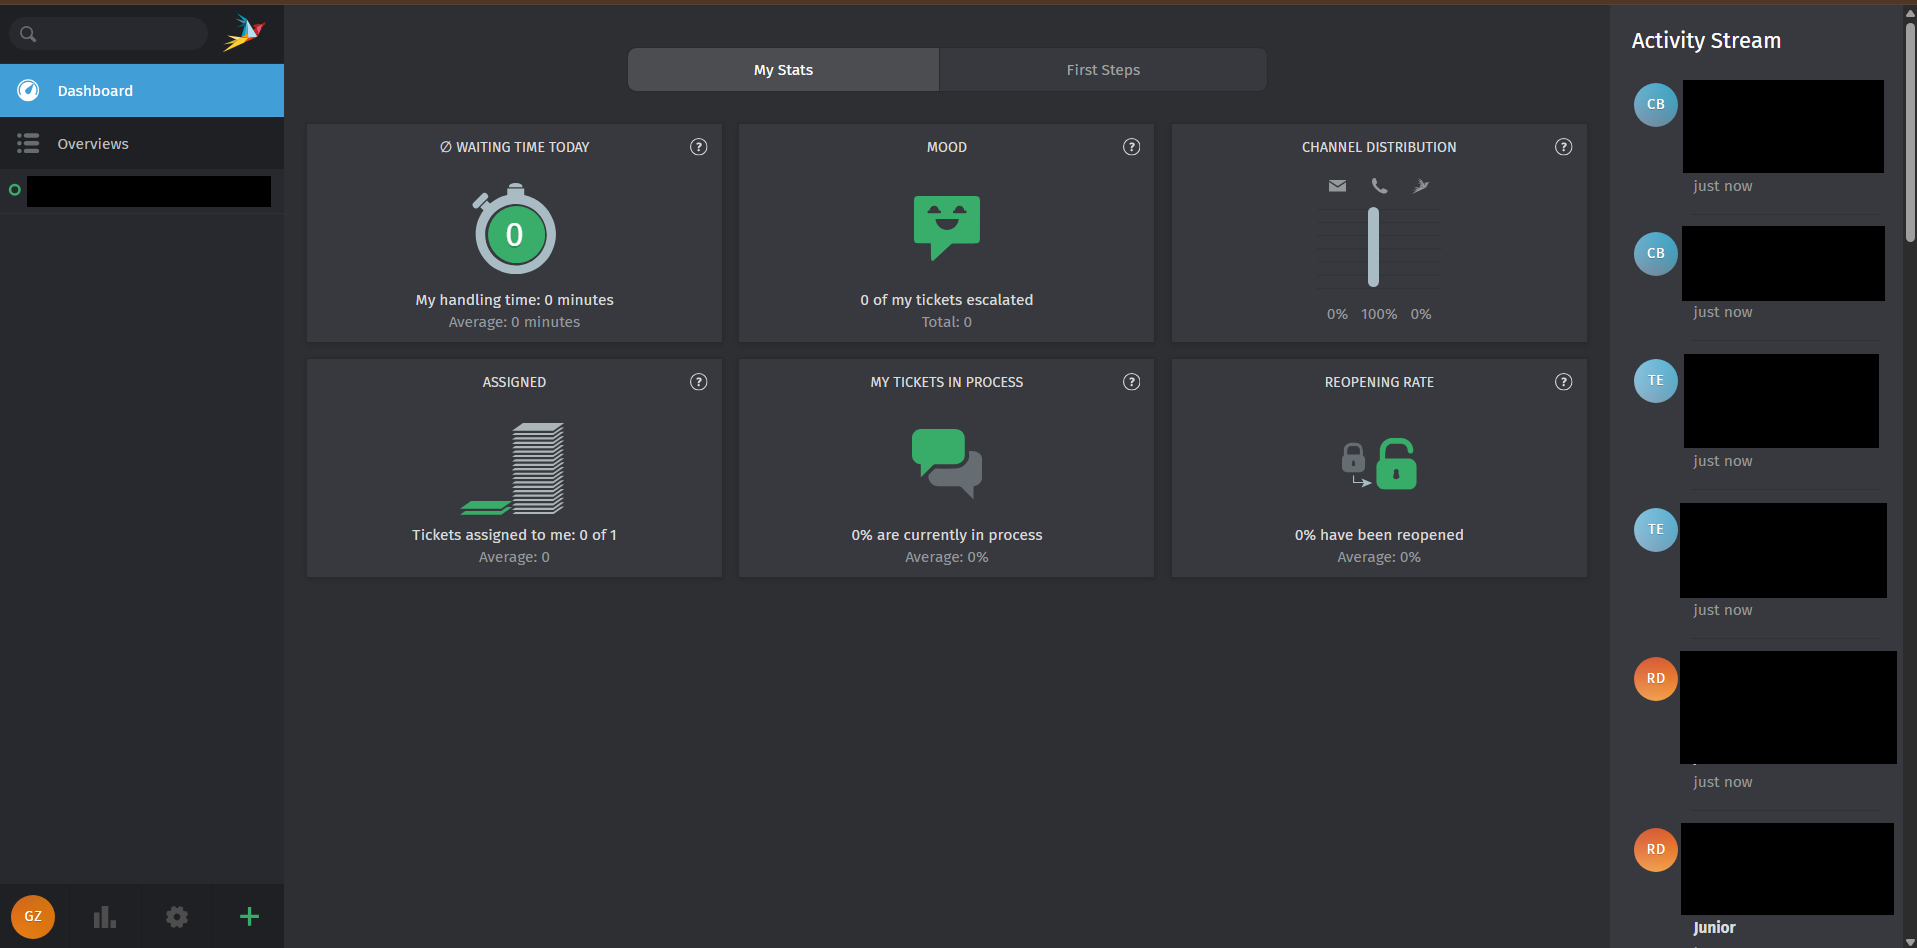
\includegraphics[width=0.8\textwidth]{Esquemas e imágenes/ZAMMAD1.png}
    \caption{Interfaz Historial de tickets Zammad}
    \label{fig:Zammad1}
\end{figure}

En el Hito 4 la integración se verificó de punta a punta con predicciones reales: a partir de la lista de riesgo del 29 de septiembre se crearon los tickets FTTH\#63002 a FTTH\#63004 en Zammad, y sus correos llegaron a una casilla de prueba a través de Azure Communication Services. El contenido del ticket y del correo se describe en la Sección~\ref{subsec:alerta}.



\section{Verificación, Validación y Testing}
\label{sec:vvt}
\noindent
verificación determina si los productos de cada etapa del desarrollo satisfacen los requisitos y 
 especificaciones establecidos para dicha etapa; en el contexto de este proyecto, si cada módulo implementa
  correctamente su diseño. La validación determina si el sistema resultante satisface el uso previsto 
  y las necesidades del usuario; en este caso, si las alertas generadas permiten a Liberty Latinamerica anticipar
   degradaciones físicas en la red FTTH con una precisión que justifique el mantenimiento preventivo de la fibra.\\

\subsection{Verificación}
\label{subsec:verificacion}

\noindent
La verificación tiene por objetivo demostrar que los datos que ingresan al modelo corresponden exactamente
 a lo especificado en el diseño. Los defectos en la limpieza rara vez producen
  errores de ejecución. No obstante, generan conjuntos de datos estructuralmente válidos pero con contenido incorrecto
  , que el modelo va incorporar de manera posterior provocando resultados defectuosos. Por este motivo, la verificación se define en
   las siguientes etapas que se describen a
    continuación.\\
    \newline
\noindent
\textbf{Carga de datos } 
\\
En el Hito 4 se leen siete fuentes: cuatro diarias de 61 días, en formato Parquet, y tres fijas en \texttt{.csv}, reutilizadas del Hito 3. Cada fuente se registra como vista de DuckDB, se filtra a registros de Panamá mediante el prefijo \texttt{PAN} del identificador de sitio y se perfila mediante
la fracción de valores nulos por columna. El Cuadro~\ref{tab:carga} resume los volúmenes que reporta el notebook antes
y después de la limpieza.

\begin{table}[htbp]
\centering
\caption{Volumen de registros por fuente en el Hito 4 (1 de agosto al 30 de septiembre de 2026), según el notebook de minería de datos}
\label{tab:carga}
\small
\renewcommand{\arraystretch}{1.25}
\begin{tabularx}{\textwidth}{|p{5.6cm}|r|>{\raggedleft\arraybackslash}p{2.7cm}|>{\raggedright\arraybackslash}X|}
\hline
\rowcolor{black}
\textcolor{white}{\textbf{Fuente}} & \textcolor{white}{\textbf{Cargados}} & \textcolor{white}{\textbf{Tras limpieza}} & \textcolor{white}{\textbf{Rol}} \\ \hline
\texttt{mosaic\_\allowbreak{}ont\_\allowbreak{}sts} (diaria) & 14.531.931 & 14.442.061 (equipo-día) & Núcleo (\texttt{serial} + \texttt{dt}) \\ \hline
\texttt{bbms\_\allowbreak{}portstats} (diaria, tres fotos por día) & 43.663.452 & 13.850.335 (puerto-día) & Integrada (día anterior) \\ \hline
\texttt{mosaic\_\allowbreak{}pon\_\allowbreak{}sts} (diaria) & 915.804 & 915.804 (puerto PON-día) & Integrada \\ \hline
\texttt{nce} (diaria, evento por evento) & 7.161.703 & 3.158.965 (alarmas únicas) & Integrada (agregada por equipo y día) \\ \hline
\texttt{cwp\_\allowbreak{}historic\_\allowbreak{}fixed\_\allowbreak{}network\_\allowbreak{}points.csv} (fija) & 1.000.000 & 147.460 (cuentas) & Integrada \\ \hline
\texttt{cwp\_\allowbreak{}Serviceabily\_\allowbreak{}HFC\_\allowbreak{}FTTH\_\allowbreak{}2024\_\allowbreak{}GAA\_\allowbreak{}2025.csv} (fija) & 63.517 & 343 (centrales) & Integrada (agregada por OLT) \\ \hline
\texttt{pca\_\allowbreak{}wsp\_\allowbreak{}feb\_\allowbreak{}abr\_\allowbreak{}2026\_\allowbreak{}detalle.csv} (fija) & 114.183 & 35.130 (cuentas) & Integrada; ninguna variable entra al modelo \\ \hline
\texttt{bbms\_\allowbreak{}subscribers\allowbreak{}dump} & --- & --- & No incluida en la entrega de agosto y septiembre \\ \hline
\end{tabularx}
\end{table}

\paragraph{Limpieza por archivo .}
Para asegurar la integridad de los datos, se aplicaron los siguientes tratamientos de limpieza y estandarización:
\begin{itemize}
    \item \textbf{Unicidad de llaves:} cada tabla queda con una sola fila por llave: equipo y día en el núcleo, puerto y día en \texttt{bbms\_portstats} (de sus tres fotos diarias se conserva la última), puerto PON y día en \texttt{mosaic\_pon\_sts} y una fila por alarma en \texttt{nce}. Ante duplicados se conserva la fila más completa (en el núcleo, la que tiene alarma crítica o mediciones) y, si dos filas empatan, un desempate fijo calculado con el contenido de la fila hace que el resultado sea idéntico en cada ejecución. En \texttt{cwp\_Serviceabily} se verifica que no haya duplicados por (\texttt{oltid}, \texttt{fdh}, \texttt{fdp}, \texttt{name}).
    \item \textbf{Eliminación de lecturas físicamente imposibles:} en \texttt{bbms\_portstats} se anulan las potencias iguales a 21.474.836 o con magnitud superior a 60 dBm. En el núcleo se anulan las lecturas de \texttt{olt\_rx} iguales a $-50$ dBm, mayores que $-8$ dBm o menores o iguales a $-40$ dBm, y las de \texttt{olt\_tx} iguales a $-50$ dBm o menores que $-10$ dBm; esas filas se marcan con \texttt{lectura\_optica\_atipica} (10.372 equipo-días). También se eliminan las filas sin errores BIP.
    \item \textbf{Vacío antes que inventado:} las mediciones vacías no se rellenan. Cuando un equipo no tiene ninguna medición se marca con \texttt{ont\_sin\_medicion} (1.601.437 equipo-días, el 11\,\%), y los modelos de árboles aprenden directamente qué hacer con el vacío. Solo las categorías del equipo (modelo, óptica y firmware) se rellenan con la moda, y los campos de servicio con ``Sin asignar''. En el Hito 3, rellenar la temperatura con la mediana hizo que el modelo la usara como señal de ``equipo sin datos''.
    \item \textbf{Fechas y horas:} \texttt{alarm\_stamp} se convierte de UTC a hora de Panamá para saber qué día empezó cada alarma. En \texttt{nce} se quita el sufijo ``GMT-05:00'' y, cuando una misma alarma aparece en dos días seguidos, se conserva el primer día en que aparece. El tiempo encendido de \texttt{bbms\_portstats} (por ejemplo, ``5d 20h 11m 10s'') se convierte a segundos.
\end{itemize}


\subsection{Validación}
\label{subsec:validacion}
\noindent
La validación evalúa la adecuación del sistema a la necesidad operativa de Liberty Latinamerica,
 formalizada en los requerimientos RF5 (entrenamiento y validación, implementada como partición en el tiempo),
  RF6 (generación de predicciones) y RF7 (cálculo de métricas), así como en el criterio de selección de M.4
   (Sección~\ref{subsec:modelo}), que privilegia el F1-Score y el área bajo la curva de precisión-cobertura (PR-AUC) 
   por sobre la exactitud.

\subsubsection{Validación ejecutada de la variable objetivo}
La definición de \textbf{falla\_optica} se contrastó contra el registro de
alarmas de NCE, un sistema de gestión de red independiente del que origina la
variable. En el Hito 3 el contraste se hizo con los cinco días de mayo; en el
Hito 4 se repitió con los 61 días de agosto y septiembre, en los que
\textbf{falla\_optica} marca 109.431 de los 14.442.061 equipo-días (0,758\,\%).
La definición deja fuera las alarmas críticas no ópticas: los cortes de energía en el
domicilio del cliente (\textit{dying gasp}) son, por sí solos, el 85,9\,\% de todas las alarmas críticas.\\\\

\noindent
El indicador de validez adoptado no es la coincidencia absoluta, sino el
enriquecimiento: la probabilidad de que un registro esté etiquetado como falla
es del 4,923\,\% cuando NCE reporta una alarma óptica ese mismo día,
frente a 0,703\,\% cuando no la reporta, lo que equivale a un factor de 7,0
(5,2 con los datos de mayo del Hito 3).
Dado que ambos sistemas no comparten el sistema en donde son capturados los datos, esta concordancia
constituye evidencia de validez de \textbf{falla\_optica}.\\\\

\noindent
El contraste se repitió admitiendo desfases de hasta dos días entre ambas
fuentes, obteniéndose factores de 7,0 ($\pm$0 días), 6,0 ($\pm$1 día) y 5,4
($\pm$2 días). El factor es máximo cuando se exige el mismo día y disminuye al
ampliar la ventana, por lo que la concordancia no proviene de una tolerancia
temporal amplia: ambas fuentes coinciden también en el día de la falla.\\\\

\noindent
Adicionalmente, se verificó que la variable es reconstruible de forma
determinista a partir de su columna de origen y que ninguna variable del mismo
día derivada de ella forma parte del conjunto de predictores. En la tarea del
Hito 4, las variables que usan el historial de fallas (por ejemplo, los días
desde la última falla) solo consideran días anteriores, y todas las demás usan
información disponible antes de la foto del día, lo que descarta la fuga de
información.

\subsubsection{Selección y validación del modelo}
\label{subsec:validacion_modelo}
\noindent
Los datos se particionaron en el tiempo (Sección~\ref{subsec:revision_diseno}).
El entrenamiento usa una muestra con todas las fallas nuevas y el 5\,\% de los
equipo-días sin falla, con peso 20. Cada semana de validación se predice con un
modelo entrenado solo con los días anteriores a ella: la primera (8 al 14 de
septiembre), con los días hasta el 7 de septiembre (363.846 filas de la
muestra y 4.593 fallas nuevas), y la segunda (15 al 21 de septiembre), con los
días hasta el 14 de septiembre (446.870 filas y 5.739 fallas nuevas). Ambas
semanas suman 3.288.133 equipo-días y 2.211 fallas nuevas. El modelo final se
reentrenó con los días hasta el 21 de septiembre y se evaluó en la semana de
prueba (22 al 29 de septiembre, 1.854.618 equipo-días y 1.213 fallas nuevas),
que no se utilizó en ninguna decisión.\\\\

\noindent
Cada modelo candidato se optimizó con Optuna, con entre 12 y 30 pruebas por
modelo y una semilla fija, y se eligió el de mayor PR-AUC promedio en las dos
semanas de validación. Se usa el PR-AUC porque no depende del número de alertas
que se emitan; el F1 se informa para el punto de operación elegido
(Sección~\ref{subsec:metricas}). El Cuadro~\ref{tab:modelos} resume la comparación.

\begin{table}[H]
\centering
\caption{Comparación de modelos candidatos en las dos semanas de validación (promedio)}
\label{tab:modelos}
\small
\renewcommand{\arraystretch}{1.3}
\begin{tabularx}{\textwidth}{|>{\raggedright\arraybackslash}X|>{\raggedright\arraybackslash}p{2.2cm}|>{\raggedright\arraybackslash}p{3cm}|>{\raggedright\arraybackslash}p{1.6cm}|>{\raggedright\arraybackslash}p{2.6cm}|}
\hline
\rowcolor{black}
\textcolor{white}{\textbf{Modelo}} & \textcolor{white}{\textbf{PR-AUC sin optimizar}} & \textcolor{white}{\textbf{PR-AUC con Optuna}} & \textcolor{white}{\textbf{Veces el azar}} & \textcolor{white}{\textbf{Precisión con 50 alertas/día}} \\ \hline
\textbf{LightGBM (elegido)} & 0,0139 & 0,0146 (+5\,\%) & 22 & 11,3\,\% \\ \hline
XGBoost & 0,0132 & 0,0142 (+8\,\%) & 21 & 10,6\,\% \\ \hline
Random Forest & 0,0084 & 0,0116 (+38\,\%) & 17 & 10,1\,\% \\ \hline
Regresión logística & 0,0076 & 0,0094 (+25\,\%) & 14 & 7,7\,\% \\ \hline
\end{tabularx}
\end{table}

\noindent
LightGBM fue el mejor modelo antes y después de optimizar, prácticamente
empatado con XGBoost. En la semana de prueba, sin embargo, la mejora de Optuna
no se sostuvo: el LightGBM sin optimizar rindió 19,4 veces el azar, frente a
17,5 del optimizado (12,5\,\% frente a 11,0\,\% de precisión con 25 alertas
diarias). La prueba no se usa para cambiar la elección, pero indica que, con
dos semanas de validación, la optimización no aporta una mejora demostrable
para LightGBM.\\\\

\noindent
El modelo aprende patrones reales: rinde 21 veces el azar en validación, frente
a 1,0 vez cuando se entrena con las etiquetas barajadas. También memoriza parte
del entrenamiento, donde rinde 165 veces el azar; por eso todas las métricas de
este informe se miden en días posteriores al entrenamiento.

\subsection{Métricas de desempeño.}
\label{subsec:metricas}
En un conjunto en el que la gran mayoría de los registros ONT-día corresponde a operación normal,
 un clasificador que asigne sistemáticamente la clase ``sin falla'' alcanza una exactitud próxima al 100\,\%
  sin detectar degradación alguna. La evaluación se basa, por tanto, en métricas definidas sobre la clase de interés.
   La \textbf{precisión} cuantifica la fracción de alertas emitidas que corresponde a fallas reales, y el
    recall la fracción de fallas reales que fueron alertadas. El F1-Score combina ambas:
\begin{equation}
    F_1 = \frac{2 \cdot P \cdot R}{P + R}
    \label{eq:f1}
\end{equation}
donde:
\begin{itemize}
    \item $P = TP/(TP + FP)$ es la precisión;
    \item $R = TP/(TP + FN)$ es el recall;
    \item $TP$ es el número de registros con falla alertados por el modelo (verdaderos positivos);
    \item $FP$ es el número de registros sin falla alertados por el modelo (falsos positivos);
    \item $FN$ es el número de registros con falla no alertados por el modelo (falsos negativos).
\end{itemize}
Dado que el F1-Score depende del umbral de decisión, se complementa con el PR-AUC, estimado mediante la precisión promedio:
\begin{equation}
    AP = \sum_{n} \left( R_n - R_{n-1} \right) P_n
    \label{eq:ap}
\end{equation}
donde $n$ indexa los umbrales de decisión ordenados de mayor a menor, $P_n$ y $R_n$ son la precisión y el recall obtenidos con el umbral $n$, y $R_0 = 0$. \\

\noindent
\textbf{Resultados en la semana de prueba.} El modelo entrega un orden de riesgo, y la decisión operativa consiste en alertar cada día los $K$ equipos de mayor riesgo. El Cuadro~\ref{tab:confusion} presenta la matriz de confusión y las métricas del LightGBM elegido con $K = 25$ y $K = 50$, acumuladas en los 8 días de la semana de prueba.

\begin{table}[H]
\centering
\caption{Matriz de confusión y métricas en la semana de prueba (22 al 29 de septiembre de 2026, 1.213 fallas nuevas)}
\label{tab:confusion}
\small
\renewcommand{\arraystretch}{1.3}
\begin{tabular}{|p{5.2cm}|r|r|}
\hline
\rowcolor{black}
\textcolor{white}{\textbf{Indicador}} & \textcolor{white}{\textbf{25 alertas/día}} & \textcolor{white}{\textbf{50 alertas/día}} \\ \hline
Verdaderos positivos ($TP$) & 22 & 37 \\ \hline
Falsos positivos ($FP$) & 178 & 363 \\ \hline
Falsos negativos ($FN$) & 1.191 & 1.176 \\ \hline
Verdaderos negativos ($TN$) & 1.853.227 & 1.853.042 \\ \hline
Precisión ($P$) & 11,00\,\% & 9,25\,\% \\ \hline
Recall ($R$) & 1,81\,\% & 3,05\,\% \\ \hline
F1-Score (ecuación~\ref{eq:f1}) & 3,11\,\% & 4,59\,\% \\ \hline
Exactitud & 99,93\,\% & 99,92\,\% \\ \hline
\end{tabular}
\end{table}

\noindent
La exactitud supera el 99,9\,\% aun cuando casi todas las fallas quedan sin alerta: un sistema que nunca alerta obtendría el mismo valor, lo que confirma por qué no se usa. El recall, y con él el F1, está acotado por construcción: con 25 alertas diarias se revisan muchos menos equipos que las cerca de 150 fallas nuevas de cada día, por lo que incluso un modelo perfecto alcanzaría un recall de 16,5\,\%. Sin depender del número de alertas, el PR-AUC en la prueba es de 0,0114, 17,5 veces el azar, y el ROC-AUC de 0,684. La lectura operativa de estos resultados se presenta en la Sección~\ref{subsec:metas}.


\subsection{Plan de Testing}
\label{subsec:testing}
\noindent
El plan de pruebas traduce las actividades anteriores en casos ejecutables. Las pruebas unitarias, de integración y de continuidad operativa.
\\
\noindent
\\
\textbf{Pruebas unitarias.}
\newline
El Cuadro~\ref{tab:unitarias} define los casos  para  las funciones de limpieza.

\begin{table}[H]
\centering
\caption{Casos de prueba unitarios sobre las reglas de limpieza del notebook}
\label{tab:unitarias}
\small
\renewcommand{\arraystretch}{1.3}
\begin{tabularx}{\textwidth}{|p{1.15cm}|p{1.2cm}|X|X|}
\hline
\rowcolor{black}
\textcolor{white}{\textbf{ID}} & \textcolor{white}{\textbf{Sección}} & \textcolor{white}{\textbf{Caso}} & \textcolor{white}{\textbf{Resultado esperado}} \\ \hline
UT-01 & 3.1 & \texttt{uptime\_a\_segundos("19d 4h 38m 14s")} & 1.658.294~s \\ \hline
UT-02 & 3.1 & \texttt{uptime\_a\_segundos} con valor nulo y con componentes omitidos (\texttt{"0d 6h 4m 26s"}) & Valor nulo; 21.866~s \\ \hline
UT-03 & 5.1 & Potencia $R_x$ igual a 21.474.836 y potencia de 75~dBm & Ambos valores anulados \\ \hline
UT-04 & 3.5 & \texttt{olt\_rx} igual a $-50$~dBm; \texttt{olt\_rx} igual a $+1{,}2$~dBm & Valor anulado \texttt{lectura\_optica\_atipica} verdadero \\ \hline
UT-05 & 3.5 & Registro con las cinco mediciones vacías; registro con una sola vacía & \texttt{ont\_sin\_medicion} verdadero sin integración; integración solo del campo vacío \\ \hline
UT-06 & 3.5 & Dos registros con igual (\texttt{serial}, \texttt{dt}), uno con alarma & Se conserva un único registro, el que tiene alarma \\ \hline
UT-07 & 3.10 & Contador BIP igual a 2.475.388.463 & \texttt{bip\_overflow\_detectado} verdadero y valor anulado \\ \hline
UT-08 & 3.9 & \texttt{parsear\_fecha\_noc("30/10/2025")} y \texttt{("3/25/2026")} & 30-10-2025 y 25-03-2026 \\ \hline
UT-09 & 3.9 & \texttt{es\_ambiguo("1/3/2026")} & Verdadero; fecha interpretada documentada \\ \hline
UT-10 & 3.8 & Expresión regular sobre \texttt{"Frame=0, Slot=13, Subslot=65535, Port=7, ONUID=35"} y sobre la misma cadena sin \texttt{ONUID} & (0, 13, 7, 35); \texttt{alarma\_nivel\_card} verdadero \\ \hline
UT-11 & 3.6 & Registro horario con conteos de servicio, advertencia e interrupción iguales a cero & Registro excluido \\ \hline
\end{tabularx}
\end{table}
\noindent
\textbf{Pruebas de integración.}
\newline
Las pruebas de integración verifican el pipeline de datos.

\begin{table}[H]
\centering
\caption{Casos de prueba de integración}
\label{tab:integracion}
\small
\renewcommand{\arraystretch}{1.3}
\begin{tabularx}{\textwidth}{|p{1.15cm}|p{1.9cm}|X|X|}
\hline
\rowcolor{black}
\textcolor{white}{\textbf{ID}} & \textcolor{white}{\textbf{Cadena}} & \textcolor{white}{\textbf{Caso}} & \textcolor{white}{\textbf{Resultado esperado}} \\ \hline
IT-01 & M.1$\rightarrow$M.2 & Ejecución completa del programa desde un núcleo reiniciado, dos veces & Sin errores; 14.442.061 equipo-días y tablas idénticas en ambas ejecuciones \\ \hline
IT-02 & M.2 & Seis uniones sobre el núcleo & Filas sin cambio y tasa de coincidencia reportada en cada unión \\ \hline
IT-03 & M.2 & Seguimiento de un conjunto de ONT de control desde el archivo de origen hasta \texttt{df\_final} & Identificadores y valores trazables en cada etapa \\ \hline
IT-04 & M.2 & Inspección de columnas de \texttt{df\_final} y de archivos exportados & Ausencia de nombres, direcciones y coordenadas de clientes (R2) \\ \hline
IT-05 & M.4$\rightarrow$M.5 & Predicción superior al umbral para un puerto PON en una instancia de prueba de Zammad & Un ticket con OLT, puerto, severidad y probabilidad \\ \hline
IT-06 & M.4$\rightarrow$M.5 & Predicciones idénticas consecutivas sobre el mismo puerto & Un único ticket (Sección~\ref{subsec:zammad}) \\ \hline
IT-07 & M.5$\rightarrow$M.6 & Ticket generado a partir de una predicción & Correo HTML sin recursos externos, con ubicación, equipo y probabilidad \\ \hline
\end{tabularx}
\end{table}

\textbf{Pruebas de continuidad operativa.} 
\newline
La señal de falla y el modelo ya están definidos. El sistema se plantea ejecutarse de forma secuencial, día a día,  y sus alertas se contrastan con los eventos efectivamente registrados, sin intervención
 sobre el entorno productivo inicialmente. Se contemplan tres casos:
\begin{itemize}
    \item \textbf{CD-01, contraste con eventos registrados:} fracción de eventos de falla precedidos por al menos una alerta y número de alertas por evento. Se ejecutó sobre la semana de prueba a nivel de equipo-día: con 25 alertas diarias, 22 de las 1.213 fallas nuevas (1,8\,\%) fueron precedidas por una alerta, es decir, unas 9 alertas por falla anticipada (Cuadro~\ref{tab:confusion}).
    \item \textbf{CD-02, revisión experta:} El jefe de operaciones (tutor) examina una muestra de alertas estratificada por severidad, que incluye falsos positivos, y registran si cada una es accionable. Esta revisión valida simultáneamente las interpretaciones de campos señaladas en la Sección~\ref{subsec:validacion}.
    \item \textbf{CD-03, legibilidad del reporte:} el usuario recibe la notificación en su dispositivo móvil y se registra si identifica equipo, ubicación y severidad sin información adicional.
\end{itemize}
Los criterios de aceptación de estas pruebas dependen de la capacidad operativa de Liberty Latinamerica, por lo que serán acordados con el tutor antes de su ejecución. 

\subsection{Análisis Crítico y Evaluación de Riesgos}
\label{subsec:riesgos_tecnicos}
\noindent
Los riesgos P1 a P3, descritos en la Sección~\ref{subsec:riesgos}, corresponden a riesgos de gestión del proyecto. El Cuadro~\ref{tab:riesgos_tecnicos} los sintetiza junto con su probabilidad e impacto estimados, las medidas de mitigación y el indicador de seguimiento.

\begin{table}[htbp]
\centering
\caption{Riesgos técnicos de implementación (P: probabilidad, I: impacto, A: alta, M: media, B: baja)}
\label{tab:riesgos_tecnicos}
\small
\renewcommand{\arraystretch}{1.3}
\begin{tabularx}{\textwidth}{|p{0.9cm}|X|p{0.4cm}|p{0.4cm}|X|X|}
\hline
\rowcolor{black}
\textcolor{white}{\textbf{ID}} & \textcolor{white}{\textbf{Riesgo}} & \textcolor{white}{\textbf{P}} & \textcolor{white}{\textbf{I}} & \textcolor{white}{\textbf{Mitigación}} & \textcolor{white}{\textbf{Indicador}} \\ \hline
RT1 & Cobertura temporal insuficiente de la telemetría de ONT & A & A & Solicitar extractos de varios meses (D1). Validar la predicción a nivel de puerto PON & Días de historia por fuente \\ \hline
RT2 & Señal de falla contaminada por eventos no ópticos & A & A & Taxonomía de alarmas validada por el tutor. Contraste con \texttt{PON.xlsx} & Correlación de rangos con la fuente independiente \\ \hline
RT3 & Exposición de datos personales (R2) & B & B & Eliminar \texttt{service\_address}. Agregar el mapa a nivel de OLT & Prueba IT-04 \\ \hline
RT4 & Fuga de información en la evaluación & M & A & Partición temporal agrupada por puerto. Exclusión de variables derivadas de la etiqueta & Diferencia entre desempeño de validación y de prueba \\ \hline
RT5 & Distorsión de la distribución óptica. & M & A & Cuantificar la fracción de datos reemplazados & Fracción de datos reemplazados por columna \\ \hline
RT6 & Uniones sin coincidencia no detectadas & M & M & Tasa de coincidencia por unión & Prueba IT-02 \\ \hline
RT7 & Ejecución no reproducible del programa & M & M & Ejecución completa desde núcleo reiniciado. & Prueba IT-01 \\ \hline
RT8 & Interpretación incorrecta de campos sin diccionario (D2) & M & M & Validación de umbrales y significados con el operador & Decisiones validadas / decisiones totales \\ \hline
RT9 & Falsos positivos y fatiga de alertas & A & A & Agregación por puerto PON. Umbral según capacidad de despacho. Control de duplicados en M.5 & Precisión operativa de los tickets \\ \hline
\end{tabularx}
\end{table}


\section{Gestión de Riesgos:}
    \label{sec:riesgos}

        \subsection{\textbf{Supuestos:}}
                    \begin{itemize}
                        \item \textbf{S1-Correlación de variables:} Se asume que existe una correlación matemática real y detectable entre los parámetros de telemetría extraídos y las degradaciones físicas de la red antes de que se conviertan en un reclamo masivo por parte de los clientes.
                        \item \textbf{S2-Representatividad histórica:} Se asume que los archivos Excel/CSV entregados por la jefatura contienen un historial de tiempo lo suficientemente amplio (muchos meses) para que el algoritmo pueda aprender los patrones estacionales y transitorios de las fallas.
                        \item \textbf{S3-Capacidad de procesamiento:} Se asume que los datos proporcionados podrán ser procesados con los recursos computacionales actuales sin requerir de una infraestructura de Big Data de alto costo.
                    \end{itemize}
        \subsection{\textbf{Dependencias:}}
                    \begin{itemize}
                        \item \textbf{D1-Entrega de datos corporativos:} El avance del cronograma depende estrictamente de que el tutor y Liberty Latinamerica proporcionen los datasets iniciales y las actualizaciones de datos en los plazos acordados.
                        \item \textbf{D2-Diccionario de datos:} Se depende de la empresa para la entrega de un glosario o diccionario de datos que explique el significado de cada columna en los archivos Excel para realizar un Feature Engineering y una reducción de dimensionalidad correctas.
                        \item \textbf{D3-Validación experta:} Se depende del conocimiento del tutor para validar si las variables que el modelo considere ``importantes'' tienen sentido físico dentro de la topología FTTH real.
                    \end{itemize}
        \subsection{\textbf{Restricciones:}} 
                    \begin{itemize}
                        \item \textbf{R1-Restricción de tiempo:} El proyecto está acotado a los plazos académicos exigidos por la universidad para la entrega de bitácoras y la defensa final de la memoria. Se considera un período de dos semestres para la entrega del prototipo final.
                        \item \textbf{R2-Confidencialidad de la información:} Al tratarse de telemetría y datos operativos de Liberty Latinamerica, existe una restricción estricta sobre la privacidad de los datos, los cuales no pueden ser expuestos públicamente y deben ser anonimizados si involucran información de clientes.
                        \item \textbf{R3-Alcance de la implementación:} El proyecto se limita al desarrollo analítico y simulación del modelo predictivo, quedando estrictamente fuera de alcance la implementación o despliegue del software en la red viva de la empresa.
                    \end{itemize}
        \subsection{\textbf{Riesgos:}}
        \label{subsec:riesgos}
                    \begin{itemize}
                        \item \textbf{P1-Calidad deficiente en los datos crudos:} Es posible que los archivos Excel entregados contengan demasiados valores nulos, formatos inconsistentes o ruido, impidiendo que el modelo aprenda correctamente. Se destinará una mayor cantidad de tiempo para el preprocesamiento e implementación de técnicas de limpieza estadística robustas.
                        \item \textbf{P2-Retraso en la entrega de la data:} Que la jefatura tarde más de lo presupuestado en extraer y enviar los datos desde los sistemas. Para mitigar este problema, se generarán datasets sintéticos con la misma estructura para programar y probar el código del pipeline antes de que los datos sean entregados por el tutor.
                        \item \textbf{P3-Desbalance de clases:} En el historial entregado existen millones de registros de red funcionando bien y muy pocos datos asociados a las fallas, haciendo que el modelo se vuelva sesgado.
                    \end{itemize}


    \section{Diseño de interfaz}
    \label{sec:interfaz}
    \noindent
    El diseño de interfaz se centra en la visualización de los resultados del modelo predictivo y distribución de datos. Se propone un sistema de notificación por correo electrónico que entrega
    reportes de posibles fallas en la red FTTH, reduciendo así la fricción cognitiva del usuario para justificar esta decisión al materializar la integración con la plataforma de ticketing Zammad. Esto garantiza
    que los técnicos y administradores de red reciban información crítica directamente en sus dispositivos móviles o en sus puestos de trabajo en el momento exacto en que se requiera su atención.

    \subsection{Modelo de Navegación}
    \noindent
    En el siguiente diagrama modela el flujo de información desde que se evalúa la anomalía hasta que la alerta es consumida por el usuario. La navegación del sistema opera de la siguiente manera:

    \begin{figure}[H]
            \centering
            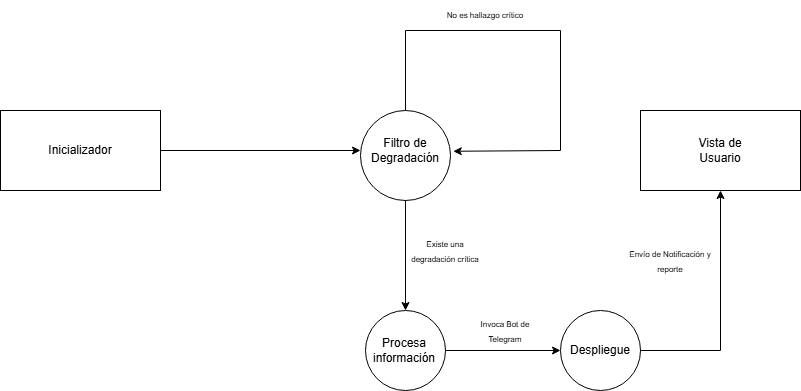
\includegraphics[width=0.8\textwidth]{Esquemas e imágenes/Modelo Navegación.png}
            \caption{Modelo de Navegación}

    \end{figure}

    \begin{itemize}
        \item \textbf{Inicializador:} El sistema comienza el proceso de evaluación de la red FTTH mediante la ejecución del modelo predictivo.
        \item \textbf{Filtro de degradación:} Es el núcleo que evalúa el modelo. En el prototipo, el modelo ordena todos los equipos según su riesgo de falla óptica nueva al día siguiente, y solo los primeros de la lista diaria (por ejemplo, 25) se consideran hallazgo crítico. Para el resto, ``No es hallazgo crítico'': el flujo se reinicia y queda a la espera de la foto del día siguiente sin interrumpir al usuario.
        \item \textbf{Procesa información:} Para los equipos que quedan en la lista del día (''Existe una degradación crítica''), los datos pasan a esta etapa, que agrega su ubicación en la red (central, puerto PON y armario) para estructurar el ticket.
        \item \textbf{Despliegue: Helpdesk:} Se activa el mecanismo de comunicación, invocando la API de Zammad.
        \item \textbf{Vista de Usuario:} El flujo concluye con el ''Envío de Notificación y reporte'' donde el usuario visualiza la alerta directamente en su cliente de mensajería o correo electrónico, cerrando el ciclo de navegación de la información.  
    \end{itemize}


\subsection{Diseño de Interfaces de Usuarios}
\noindent
La interfaz de usuario final se ha diseñado pensando en la inmediatez, aprovechando la vista móvil de las aplicaciones de correo electrónico a través de la integración automatizada con Zammad. El diseño carece de elementos distractivos y prioriza una jerarquía visual orientada a la rápida asimilación de la información técnica crítica.

\begin{figure}[H]
    \centering
    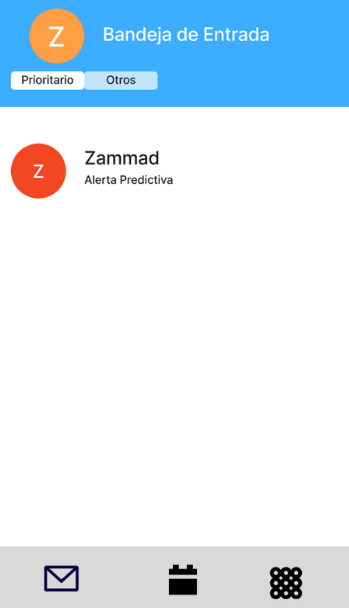
\includegraphics[width=0.4\textwidth]{Esquemas e imágenes/Interfaz 1.png}
    \caption{Vista principal de notificación preventiva de Zammad en la bandeja de entrada (maqueta).}
    \label{fig:interfaz1}
\end{figure}

\begin{figure}[H]
    \centering
    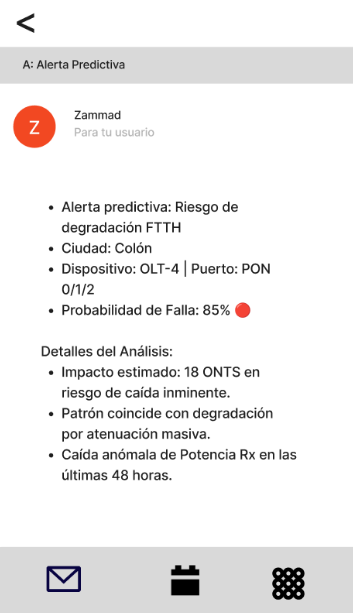
\includegraphics[width=0.4\textwidth]{Esquemas e imágenes/Interfaz 2.png}
    \caption{Reporte detallado tras la apertura de la notificación en el cliente de correo (maqueta).}
    \label{fig:interfaz2}
\end{figure}

\noindent
Las Figuras~\ref{fig:interfaz1} y~\ref{fig:interfaz2} corresponden a la maqueta de diseño de la notificación, y sus valores son ilustrativos. El ticket implementado en el prototipo, con un ejemplo real, se describe en la Sección~\ref{subsec:alerta}. Los elementos de la notificación y sus diferencias con la maqueta son los siguientes:

\begin{itemize}
    \item \textbf{Bandeja de entrada:} La alerta se identifica claramente bajo el remitente del sistema de tickets y un asunto prioritario (``Alerta predictiva''), destacándose inmediatamente frente a los correos operativos regulares.
    
    \item \textbf{Cuerpo de la Alerta:} Una vez abierto el correo, la interfaz presenta un resumen en formato de lista para agilizar la lectura técnica y la toma de decisiones:
    \begin{itemize}
        \item \textbf{Contexto de la falla:} Se especifica de inmediato que se trata de un riesgo de falla óptica nueva para el día siguiente.
        \item \textbf{Ubicación y Hardware:} Se expone la ubicación del equipo en la red: equipo del cliente, central (OLT), puerto PON y, cuando la tabla de topología lo permite, el armario de distribución (en el ejemplo real: central PAN-LMT-CPO-PHM001, puerto PON 0/16/15 y armario CPG-015). La maqueta mostraba la ciudad (Ej. Colón); el ticket implementado la reemplaza por el armario, que orienta mejor las salidas o el despliegue de personal técnico a zona.
        \item \textbf{Métrica de riesgo:} Se destaca la probabilidad de falla óptica nueva para el día siguiente y el puesto del equipo en la lista del día. El 85\,\% de la maqueta es ilustrativo: como en promedio solo 1 de cada 1.540 equipo-días presenta una falla nueva, los riesgos reales son mucho menores (el más alto del ejemplo real es 25,3\,\%), por lo que la prioridad se expresa con el orden de la lista y no con un umbral fijo.  
    \end{itemize}

    \item \textbf{Detalles del Análisis:} Sección dedicada a la explicabilidad del modelo predictivo, fundamental para generar confianza en el usuario. En lugar del impacto estimado y del patrón que mostraba la maqueta, se presentarán los motivos principales de cada alerta, calculados con valores SHAP (por ejemplo, alarmas ópticas de la semana, aumento de errores de bit y fallas recientes). Estos motivos ya se calculan, pero aún no se incluyen en el ticket (Sección~\ref{subsec:alerta}).
\end{itemize}



%==================================================================
%  HITO 4: PROTOTIPO COMERCIAL (PrediFibra)
%==================================================================
% Columnas alineadas a la izquierda para las tablas de esta sección
\newcolumntype{Q}[1]{>{\raggedright\arraybackslash}p{#1}}
\newcolumntype{Z}{>{\raggedright\arraybackslash}X}
\section{Prototipo comercial: PrediFibra}
\label{sec:predifibra}
\noindent
En el Hito 4 el prototipo deja de evaluarse solo como un desarrollo técnico y se presenta como un producto que un operador FTTH puede contratar. Ese producto se denomina \textbf{PrediFibra}, y su propuesta comercial se desarrolla en el Plan de Negocios de PrediFibra SpA, elaborado en paralelo en el módulo de Plan de Negocios de las Memorias Transversales. Esta sección resume los avances técnicos que sostienen la oferta (Sección~\ref{subsec:avances_h4}); qué se ofrece y a quién (Secciones~\ref{subsec:oferta} y~\ref{subsec:valor}); cómo funciona la plataforma en la nube y qué recibe el usuario (Secciones~\ref{subsec:arq_azure} y~\ref{subsec:alerta}); cuánto cuesta operarla (Sección~\ref{subsec:costos}); cómo se compara su desempeño con las metas del plan (Sección~\ref{subsec:metas}), y cuáles son sus límites y próximos pasos (Sección~\ref{subsec:hoja_ruta}).

%------------------------------------------------------------------
\subsection{Avances técnicos desde el Hito 3}
\label{subsec:avances_h4}
\noindent
El Cuadro~\ref{tab:h3_h4} resume los cambios entre el prototipo presentado en el Hito 3 y el que respalda la oferta comercial. El cambio central es la tarea: en el Hito 3 se buscaba detectar fallas ópticas en curso; en el Hito 4 el modelo \textbf{anticipa} las fallas ópticas nuevas (LOSi, LOBi, LOFi o fibra de distribución cortada) que aparecerán en la foto de la red del día siguiente, en equipos que hoy funcionan sin alarma óptica. Los cortes de energía en el domicilio del cliente (\textit{dying gasp}) se excluyen, por ser ajenos a la red.

\begin{table}[!htb]
\centering
\caption{Avances del prototipo entre el Hito 3 y el Hito 4}
\label{tab:h3_h4}
\small
\renewcommand{\arraystretch}{1.3}
\begin{tabularx}{\textwidth}{|Q{2.9cm}|Z|Z|}
\hline
\rowcolor{black}
\textcolor{white}{\textbf{Aspecto}} & \textcolor{white}{\textbf{Hito 3}} & \textcolor{white}{\textbf{Hito 4}} \\ \hline
Datos & Cinco días de mayo de 2026: 999.766 registros ONT-día y 99 variables & 61 días (1 de agosto al 30 de septiembre de 2026): 14.442.061 equipo-días de 279.964 equipos, procesados con DuckDB y archivos Parquet \\ \hline
Tarea & Detección de fallas ópticas en curso & Anticipación de fallas ópticas nuevas para el día siguiente: 8.017 casos en 12.343.745 equipo-días (1 de cada 1.540) \\ \hline
Variables & 99 columnas del conjunto unificado & 47 variables candidatas; se eligieron 25, el menor conjunto que conserva el 97\,\% del PR-AUC obtenido con todas \\ \hline
Modelo & Entrenamientos exploratorios con Random Forest y LightGBM, sin modelo elegido & Regresión logística, Random Forest, XGBoost y LightGBM, optimizados con Optuna; se eligió LightGBM por su desempeño en dos semanas de validación \\ \hline
Evaluación & Partición por dispositivo, con fines exploratorios & Partición en el tiempo: entrenamiento desde el 8 de agosto, dos semanas de validación (8 al 21 de septiembre) y una semana de prueba nunca vista (22 al 29 de septiembre) \\ \hline
Reproducibilidad & Resultados con leves variaciones entre ejecuciones & Ejecución reproducible: desempates fijos en la limpieza y número fijo de pruebas en Optuna \\ \hline
Notificación & Zammad en un contenedor Docker, conectado por API REST y a la espera de predicciones & Plataforma desplegada en Azure y conectada de punta a punta: la lista diaria de riesgo genera tickets en Zammad y correos al equipo de IT \\ \hline
\end{tabularx}
\end{table}

%------------------------------------------------------------------
\subsection{PrediFibra: qué es, para quién y cómo se ofrece}
\label{subsec:oferta}
\noindent
PrediFibra es el nombre comercial del prototipo, acompañado del eslogan \textit{``Mantenimiento predictivo para redes FTTH''}. Su misión, tal como la define el Plan de Negocios, es anticipar las fallas de las redes de fibra óptica antes de que las sufran sus usuarios, entregando a los operadores FTTH de Latinoamérica una plataforma predictiva simple, independiente del fabricante y a un precio que un operador mediano puede pagar.\\\\

\noindent
En términos de producto, PrediFibra toma la foto diaria de la red que el operador ya genera (potencia óptica de OLT y ONT, alarmas ópticas y errores de transmisión), calcula para cada equipo la probabilidad de una falla óptica nueva al día siguiente y entrega cada mañana una lista priorizada de tickets de mantenimiento preventivo. Es solo software: no requiere instalar sondas, OTDR ni otro equipamiento en las centrales. El cliente es una empresa, por lo que se distingue entre quien decide la compra y quien usa el producto:
\begin{itemize}
    \item \textbf{Quién compra:} el gerente o director de operaciones de red, de ingeniería de acceso fijo o del NOC de un operador FTTH, que responde por indicadores como cortes por cada mil clientes, tiempo de reparación y costo de las visitas técnicas.
    \item \textbf{Quién usa:} los ingenieros del NOC, que reciben y priorizan los tickets preventivos, y el personal técnico encargado de las salidas o el despliegue a zona para revisar los equipos alertados.
\end{itemize}

\noindent
El Plan de Negocios define tres segmentos, en orden de prioridad: (1) operadores medianos y regionales de Chile, de entre 20.000 y 1.000.000 de accesos de fibra, con redes en expansión y sin un equipo propio de ciencia de datos; (2) las operaciones de Liberty Latin America en Latinoamérica y el Caribe, contraparte de este desafío, donde cada país opera como una unidad de negocio que puede contratar su propia licencia; y (3) otros operadores FTTH de la región a partir del tercer año. La oferta se estructura en tres productos que se contratan en secuencia (Cuadro~\ref{tab:oferta}).

\begin{table}[!htb]
\centering
\caption{Oferta comercial de PrediFibra (precios netos de IVA, Año 1 del Plan de Negocios)}
\label{tab:oferta}
\small
\renewcommand{\arraystretch}{1.3}
\begin{tabularx}{\textwidth}{|Q{3.2cm}|Z|Q{2.8cm}|}
\hline
\rowcolor{black}
\textcolor{white}{\textbf{Producto}} & \textcolor{white}{\textbf{Qué incluye}} & \textcolor{white}{\textbf{Precio (USD)}} \\ \hline
Piloto pagado (prueba de concepto) & Tres meses de operación sobre los datos del propio operador, con evaluación semanal de los resultados y un informe final. Permite medir el valor en la red del cliente antes de comprar & 8.000 por piloto \\ \hline
Licencia y despliegue & Instalación de la plataforma para un operador o una unidad de negocio (por ejemplo, un país de Liberty Latin America), conexión a sus fuentes de datos y ajuste del modelo a su red & 90.000, pago único \\ \hline
Suscripción a soporte y plataforma & Operación diaria de la plataforma, reentrenamiento del modelo y soporte, mientras el cliente usa el servicio & 18.000 al año (1.500 al mes) \\ \hline
\end{tabularx}
\end{table}

%------------------------------------------------------------------
\subsection{Propuesta de valor y diferenciación}
\label{subsec:valor}
\noindent
Hoy el mantenimiento de la red de acceso es reactivo: el operador se entera de una falla cuando aparece la alarma o cuando el cliente reclama, y la visita técnica es correctiva. PrediFibra entrega cada mañana los equipos con mayor riesgo de una falla óptica nueva al día siguiente, de modo que el NOC pueda revisar de forma remota o coordinar una salida a zona antes de que el cliente perciba el problema. En la semana de prueba (Sección~\ref{subsec:metas}), los resultados que sostienen esa propuesta son:
\begin{itemize}
    \item \textbf{Concentra el riesgo.} Con 25 alertas diarias, el 11,0\,\% corresponde a una falla nueva al día siguiente (1 de cada 9), frente a 0,065\,\% al azar (1 de cada 1.529): las alertas concentran las fallas unas 168 veces más que una selección al azar.
    \item \textbf{Supera a la práctica actual.} La mejor regla simple, que alerta a los equipos que fallaron en los 30 días previos, acierta 5,5\,\% (1 de cada 18). El modelo duplica esa precisión.
    \item \textbf{Aciertos con margen de acción.} Si se acepta una falla nueva dentro de los 3 días siguientes, acierta 1 de cada 6 alertas (17,3\,\%).
    \item \textbf{Volumen operable.} Con 25 alertas diarias (unas 750 al mes), se anticiparían unas 80 fallas nuevas al mes para el día siguiente y unas 130 dentro de 3 días. Con el costo de nube de la Sección~\ref{subsec:costos}, cada falla anticipada cuesta menos de 1 USD de infraestructura.
    \item \textbf{Ubica la falla.} Cada alerta indica el equipo, la central, el puerto PON y, cuando la topología lo permite, el armario de distribución al que enviar al personal técnico (Sección~\ref{subsec:alerta}).
\end{itemize}

\noindent
El Plan de Negocios identifica cuatro ventajas competitivas: (1) \textbf{independencia del fabricante}, ya que PrediFibra no vende equipos y se conecta a la telemetría que el operador ya tiene; (2) \textbf{solo software}, sin sondas ni obras en las centrales; (3) \textbf{un equipo} que combina ciencia de datos, infraestructura en la nube y operación de redes fijas; y (4) \textbf{una barrera de entrada baja}, porque el piloto pagado permite medir el valor en la red propia antes de comprometer una licencia. El Cuadro~\ref{tab:competencia} sitúa la oferta frente a los tres tipos de competidores identificados en el plan. El competidor más directo es Adtran Mosaic One Clarity, que ofrece mantenimiento predictivo con inteligencia artificial y con el que uno de sus primeros clientes proyecta hasta un 75\,\% menos de tickets de falla al mes \cite{adtran_clarity}. PrediFibra no se diferencia por una tecnología exclusiva, sino por su foco en operadores medianos de Latinoamérica, su precio de entrada y su soporte local. Los fabricantes no publican sus precios, por lo que los valores de referencia son estimaciones del equipo que deben validarse con cotizaciones reales.

\begin{table}[!htb]
\centering
\caption{Competencia y diferenciación (fuentes: Plan de Negocios de PrediFibra y sitios de los fabricantes; precios estimados por el equipo)}
\label{tab:competencia}
\small
\renewcommand{\arraystretch}{1.3}
\begin{tabularx}{\textwidth}{|Q{3.3cm}|Z|Q{2.6cm}|Z|}
\hline
\rowcolor{black}
\textcolor{white}{\textbf{Competidor}} & \textcolor{white}{\textbf{Qué ofrece}} & \textcolor{white}{\textbf{Precio ref. (USD)}} & \textcolor{white}{\textbf{Diferencia de PrediFibra}} \\ \hline
Suites de fabricantes con IA (Nokia Altiplano AI \cite{nokia_altiplano}, Adtran Mosaic One Clarity \cite{adtran_clarity}) & IA sobre la telemetría de la red y automatización, vendidas junto con proyectos de equipamiento & $\sim$150.000 al año & No depende del fabricante de la OLT y se vende a operadores medianos \\ \hline
Monitoreo óptico con hardware (EXFO \cite{exfo_pon}, VIAVI \cite{viavi_onms}, Adtran ALM \cite{adtran_alm}) & Detección de fallas físicas en la fibra con sondas y OTDR instalados en las centrales & $\sim$120.000 (equipos y software) & No instala hardware: usa la telemetría existente \\ \hline
Consultoras de analítica y equipos internos & Desarrollo a medida para un operador & $\sim$60.000 por proyecto & Producto replicable, con piloto de precio acotado \\ \hline
\textbf{PrediFibra} & Predicción independiente del fabricante, solo software, con piloto pagado & 8.000 piloto; 90.000 licencia; 18.000 al año & --- \\ \hline
\end{tabularx}
\end{table}

%------------------------------------------------------------------
\subsection{Arquitectura del prototipo en Azure}
\label{subsec:arq_azure}
\noindent
La plataforma se implementó en Microsoft Azure y se encuentra conectada de punta a punta, desde la recepción de la foto diaria hasta la creación del ticket y el envío del correo. Está diseñada para desplegarse en la suscripción de Azure que el operador ya utiliza. La Figura~\ref{fig:arq_azure} muestra sus seis etapas, que corresponden a los módulos M.1 a M.6 de la arquitectura de la Figura~\ref{MODELO ML}, ahora ejecutados de forma diaria en la nube.

\begin{figure}[!htb]
    \centering
    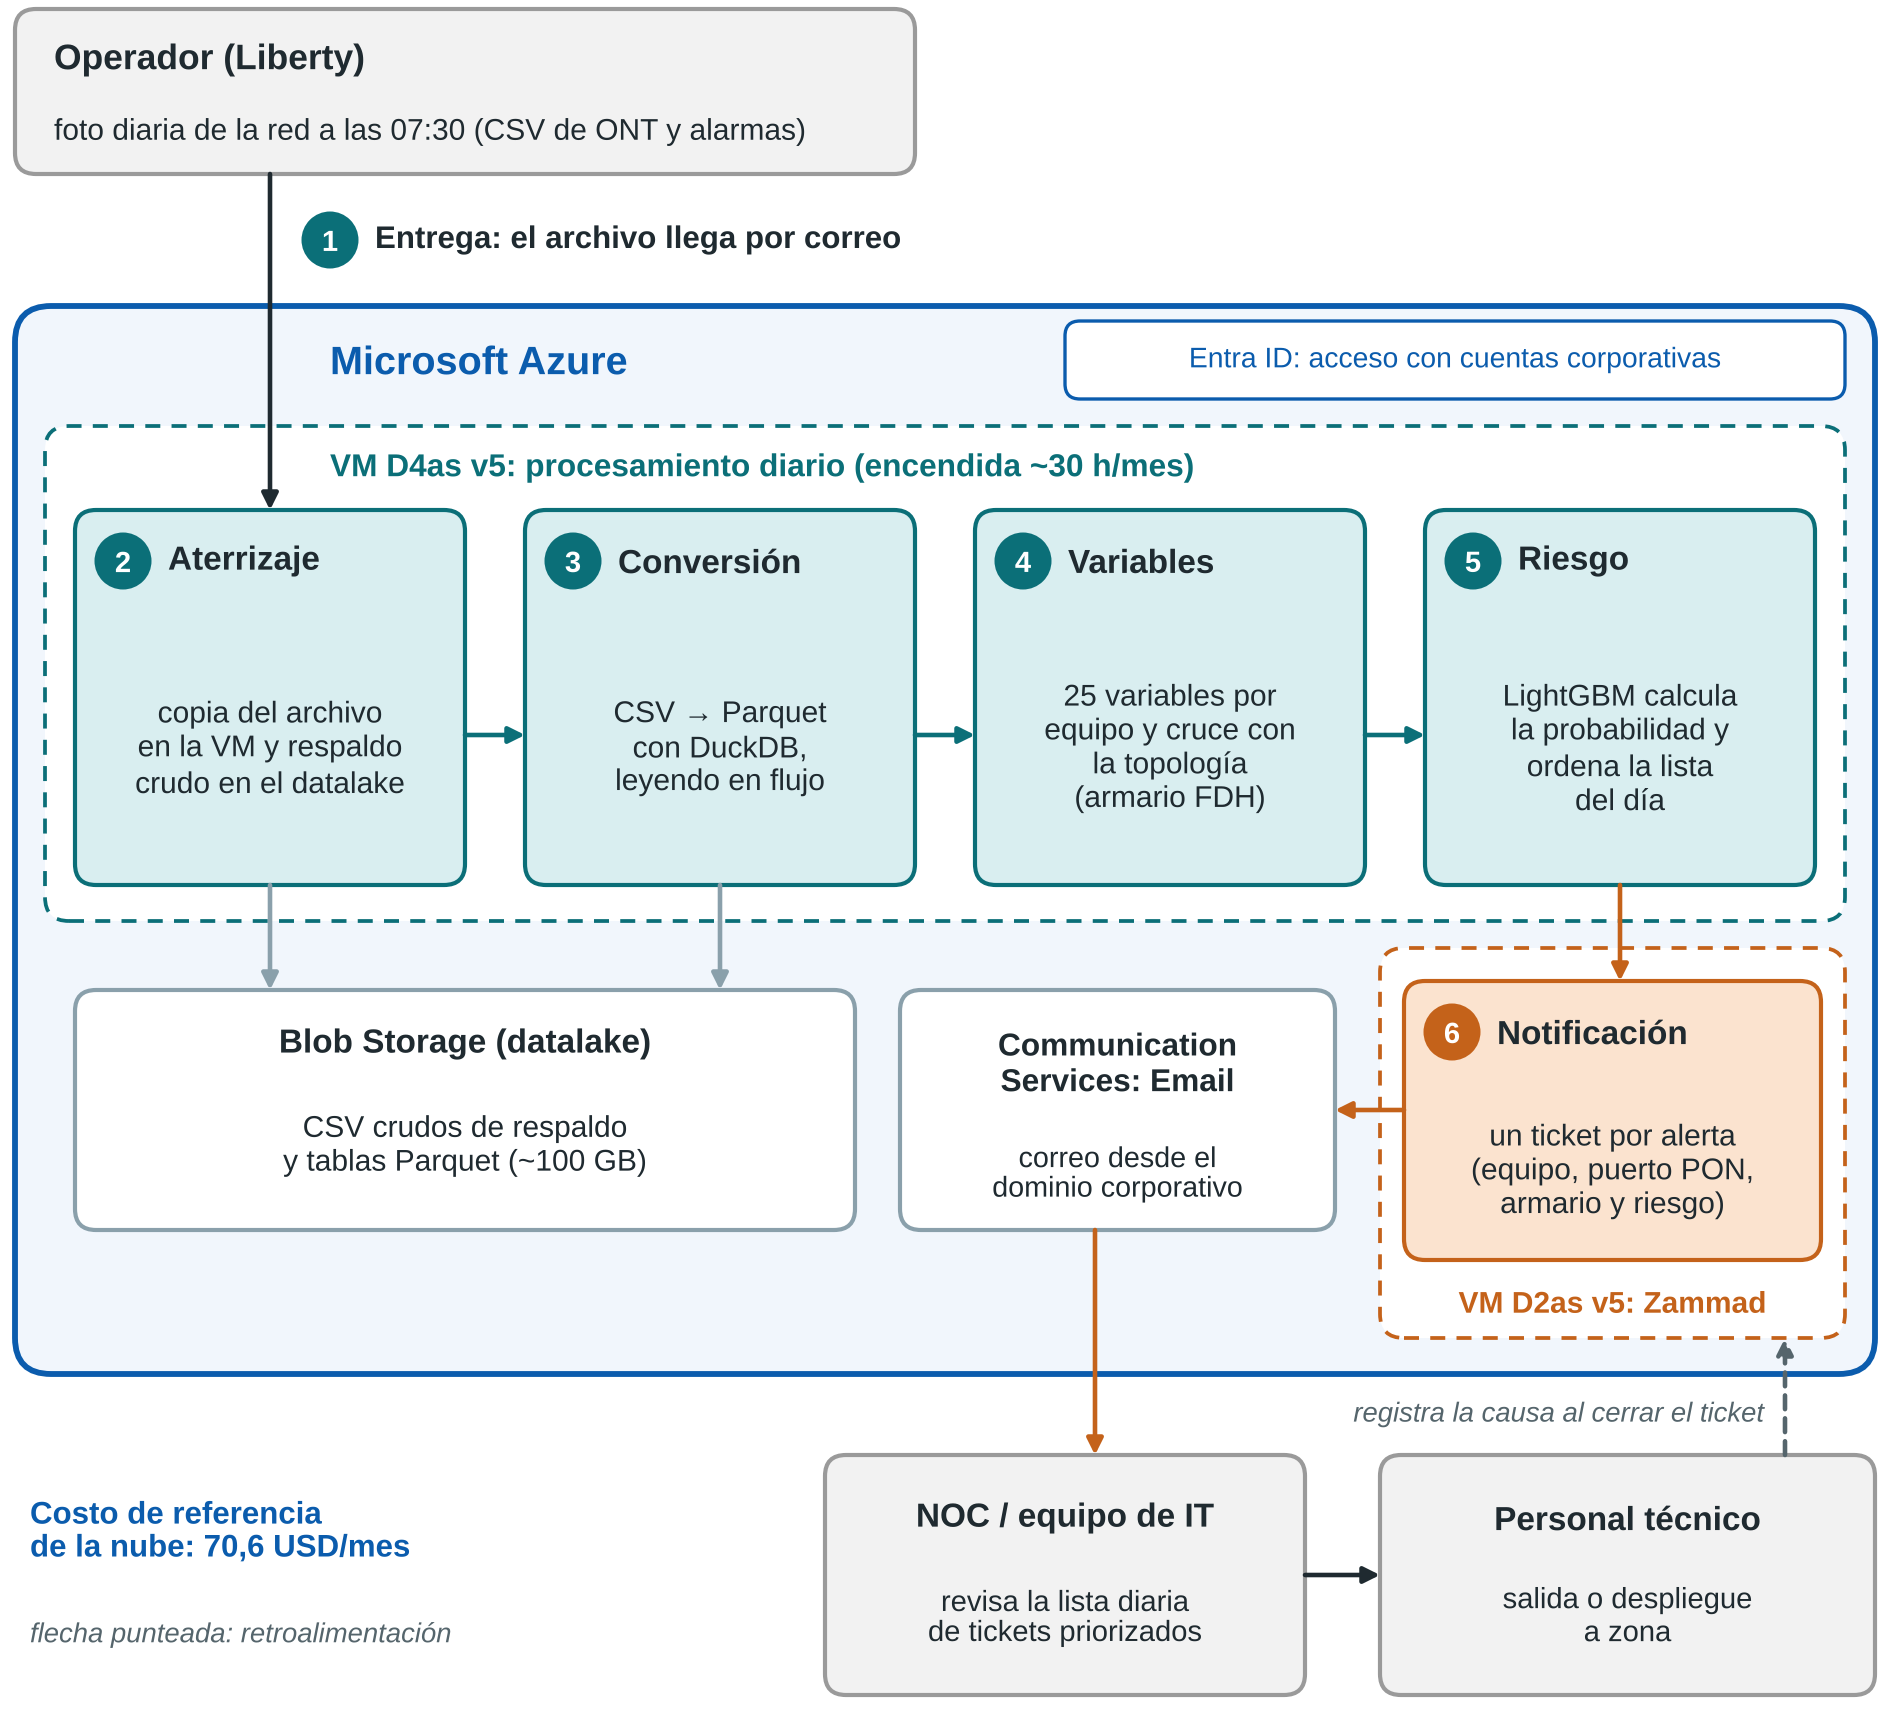
\includegraphics[width=\textwidth]{Esquemas e imágenes/Arquitectura Azure PrediFibra.png}
    \caption{Arquitectura del prototipo PrediFibra en Microsoft Azure}
    \label{fig:arq_azure}
\end{figure}

\begin{enumerate}
    \item \textbf{Entrega (M.1):} el operador envía por correo la foto diaria de la red, generada a las 07:30.
    \item \textbf{Aterrizaje (M.1):} el archivo se copia en la máquina virtual de procesamiento y se guarda un respaldo crudo en el \textit{datalake} (Blob Storage).
    \item \textbf{Conversión (M.2):} los CSV se convierten a Parquet con DuckDB, leyéndolos en flujo, sin cargar todo el archivo en memoria.
    \item \textbf{Variables (M.3):} se calculan las 25 variables del modelo con el mismo código del notebook de entrenamiento, y se cruza la topología del cliente para resolver el armario de distribución de cada equipo.
    \item \textbf{Riesgo (M.4):} el modelo LightGBM entrega la probabilidad de falla óptica nueva de cada equipo y ordena la lista del día.
    \item \textbf{Notificación (M.5 y M.6):} se crea un ticket por alerta en Zammad y se envía un correo al equipo de IT desde el dominio corporativo del operador.
\end{enumerate}

\noindent
La máquina virtual de procesamiento se enciende solo durante la corrida diaria (unas 30 horas al mes), mientras que la de Zammad permanece siempre encendida. El acceso del personal se controla con Microsoft Entra ID, usando las mismas cuentas corporativas del operador. El diseño del ticket contempla que, al cerrarlo, el técnico registre la causa encontrada; ese registro es la retroalimentación que permitirá reentrenar el modelo con casos confirmados en terreno.

%------------------------------------------------------------------
\subsection{Diseño de la alerta}
\label{subsec:alerta}
\noindent
El equipo de IT no recibe una probabilidad aislada, sino un equipo, una ubicación en la red y un riesgo. El Cuadro~\ref{tab:ticket} muestra los campos del ticket con una alerta real de la plataforma; la serie del equipo se muestra parcialmente oculta para resguardar los datos del cliente.

\begin{table}[!htb]
\centering
\caption{Campos del ticket de alerta preventiva (ejemplo real)}
\label{tab:ticket}
\small
\renewcommand{\arraystretch}{1.3}
\begin{tabularx}{\textwidth}{|Q{3.2cm}|Q{4.6cm}|Z|}
\hline
\rowcolor{black}
\textcolor{white}{\textbf{Campo}} & \textcolor{white}{\textbf{Ejemplo}} & \textcolor{white}{\textbf{Para qué sirve}} \\ \hline
Equipo del cliente & HG8145X7-10, serie \texttt{HWTC****08B8} & Identificar la ONT alertada \\ \hline
Central (OLT) & \texttt{PAN-LMT-CPO-PHM001} & Saber desde qué central se atiende el equipo \\ \hline
Puerto PON & 0/16/15, ONU 2 & Ubicar el equipo en la red y revisar si otros equipos del puerto están afectados \\ \hline
Armario FDH & CPG-015 & Definir a qué armario de distribución dirigir la salida a zona \\ \hline
Riesgo para mañana & 25,3\,\%, el más alto de la lista del día & Priorizar las revisiones del día \\ \hline
Causa encontrada & Se completa al cerrar el ticket & Confirmar el hallazgo y alimentar el reentrenamiento \\ \hline
\end{tabularx}
\end{table}

\noindent
El armario se obtiene cruzando el puerto PON con la tabla de topología entregada por el cliente. Esa tabla cubre 97 de las 178 centrales, por lo que hoy el 24,6\,\% de las alertas llega con el armario resuelto; en las demás el ticket indica ``armario: sin dato''. Aumentar esa cobertura depende de completar la tabla de topología, no de un nuevo desarrollo.\\\\

\noindent
Uno de los valores declarados en el Plan de Negocios es la transparencia: cada ticket debe explicar por qué se generó, para que el técnico confíe en la recomendación. El modelo ya permite calcular esos motivos con valores SHAP, aunque todavía no se incluyen en el ticket. Por ejemplo, el 29 de septiembre un equipo quedó en el puesto 5 de la lista, con un riesgo de 27,9\,\%, y sus motivos principales fueron: 7 alarmas ópticas en NCE durante la semana, un aumento de 307.348 errores de bit de subida desde el día anterior, una falla ocurrida el día anterior y 29 días con falla en el último mes. Al día siguiente, ese equipo tuvo efectivamente una falla nueva. Incorporar estos motivos al ticket es parte de la hoja de ruta (Sección~\ref{subsec:hoja_ruta}).

%------------------------------------------------------------------
\subsection{Costos de operación en Azure}
\label{subsec:costos}
\noindent
El Cuadro~\ref{tab:costos_azure} detalla el costo mensual estimado de operar la plataforma en Azure, que asciende a \textbf{70,6 USD al mes}. El cálculo considera solo la infraestructura de nube para un cliente en operación; no incluye las horas del equipo (desarrollo, despliegue ni soporte).

\begin{table}[!htb]
\centering
\caption{Costo mensual estimado de la plataforma en Microsoft Azure}
\label{tab:costos_azure}
\small
\renewcommand{\arraystretch}{1.3}
\begin{tabularx}{\textwidth}{|Q{4.6cm}|Z|Q{2.2cm}|}
\hline
\rowcolor{black}
\textcolor{white}{\textbf{Servicio}} & \textcolor{white}{\textbf{Para qué se usa}} & \textcolor{white}{\textbf{USD al mes}} \\ \hline
Virtual Machines, D4as v5 & Corrida diaria del procesamiento y del modelo, 30 horas al mes & 5,2 \\ \hline
Virtual Machines, D2as v5 & Servidor de tickets Zammad, siempre encendido & 62,8 \\ \hline
Blob Storage & 100 GB de datos crudos y procesados & 1,8 \\ \hline
Communication Services, Email & 1.500 notificaciones al mes & 0,4 \\ \hline
Transferencia de salida & 5 GB al mes & 0,4 \\ \hline
Microsoft Entra ID & Identidad y control de acceso del personal & Incluido \\ \hline
\textbf{Costo operativo mensual} & \textbf{Operación completa, sin desarrollo} & \textbf{70,6} \\ \hline
\end{tabularx}
\end{table}

\noindent
La misma arquitectura se cotizó en Amazon Web Services (71,2 USD al mes) y en Google Cloud (84,4 USD al mes). En Google Cloud el costo es mayor porque el envío de correos debe contratarse a un proveedor externo (SendGrid o Mailgun, unos 15 USD al mes), lo que suma una cuarta empresa a la cadena. Se eligió Azure por razones operativas más que de precio:
\begin{itemize}
    \item \textbf{El cliente ya opera sobre Microsoft:} el correo corporativo y Entra ID de Liberty están en producción, por lo que la plataforma se despliega en la suscripción existente, sin incorporar un proveedor nuevo.
    \item \textbf{El correo sale del mismo dominio:} las notificaciones se envían con el dominio propio del operador y con sus registros de autenticación, lo que evita que lleguen como correo no deseado.
    \item \textbf{La diferencia de costo es menor:} Azure es menos de 1\,\% más barato que AWS y cerca de 16\,\% más barato que Google Cloud.
\end{itemize}

\noindent
Llevado a un semestre, el costo de nube es de 423,6 USD por cliente, dentro de los 500 USD por semestre que el Plan de Negocios asigna como costo de plataforma de cada suscripción. El servidor de Zammad explica el 89\,\% del costo mensual (62,8 de 70,6 USD): si un operador ya cuenta con su propio sistema de tickets y se integra con él, el costo de nube bajaría a unos 8 USD al mes.

%------------------------------------------------------------------
\subsection{Desempeño frente a las metas del Plan de Negocios}
\label{subsec:metas}
\noindent
Los resultados se midieron en la semana de prueba del 22 al 29 de septiembre de 2026, que el modelo no utilizó en ninguna etapa de entrenamiento ni de selección: 1.854.618 equipo-días y 1.213 fallas ópticas nuevas. En esa semana el modelo ordena los equipos 17,5 veces mejor que el azar (PR-AUC de 0,0114; ROC-AUC de 0,684). El Cuadro~\ref{tab:resultados_h4} traduce ese resultado a la operación, según el número de alertas que se revisen cada día.

\begin{table}[!htb]
\centering
\caption{Resultados en la semana de prueba (22 al 29 de septiembre de 2026)}
\label{tab:resultados_h4}
\small
\renewcommand{\arraystretch}{1.3}
\begin{tabularx}{\textwidth}{|Q{2.4cm}|Z|Z|Z|}
\hline
\rowcolor{black}
\textcolor{white}{\textbf{Alertas por día}} & \textcolor{white}{\textbf{Precisión al día siguiente}} & \textcolor{white}{\textbf{Precisión dentro de 3 días}$^{*}$} & \textcolor{white}{\textbf{Fallas anticipadas (de 1.213)}} \\ \hline
25 & 11,0\,\% (1 de cada 9) & 17,3\,\% (1 de cada 6) & 22 (1,8\,\%) \\ \hline
50 & 9,3\,\% (1 de cada 11) & 16,7\,\% & 37 (3,1\,\%) \\ \hline
100 & 6,9\,\% (1 de cada 14) & 14,2\,\% & 55 (4,5\,\%) \\ \hline
\end{tabularx}

\vspace{1mm}
\parbox{\textwidth}{\footnotesize Referencias con 25 alertas diarias: regla de fallas en los 30 días previos, 5,5\,\% (1 de cada 18); azar, 0,065\,\% (1 de cada 1.529).\\
$^{*}$ Medida del 22 al 27 de septiembre, los días de la semana con tres días siguientes observables.}
\end{table}

\noindent
Además, el modelo pierde solo un 7\,\% de PR-AUC en centrales (OLT) que nunca vio y un 2\,\% en puertos PON nuevos, lo que indica que puede extenderse a otras zonas de la red.\\\\

\noindent
El Plan de Negocios fijó sus metas técnicas antes de contar con resultados, y el propio plan las declara como metas de diseño que el piloto debe confirmar. Los resultados actuales están por debajo de esas metas, por lo que se proponen metas realistas para el piloto, que se revisarán con los datos que este genere (Cuadro~\ref{tab:metas}).

\begin{table}[!htb]
\centering
\caption{Metas del Plan de Negocios, resultados actuales y metas propuestas para el piloto}
\label{tab:metas}
\small
\renewcommand{\arraystretch}{1.3}
\begin{tabularx}{\textwidth}{|Q{2.2cm}|Q{2.3cm}|Z|Z|}
\hline
\rowcolor{black}
\textcolor{white}{\textbf{Indicador}} & \textcolor{white}{\textbf{Meta del plan}} & \textcolor{white}{\textbf{Resultado actual}} & \textcolor{white}{\textbf{Meta propuesta para el piloto}} \\ \hline
Anticipación & 7 días & 1 día (falla en la foto de mañana) & 1 a 3 días \\ \hline
Precisión & $\geq$\,60\,\% & 11,0\,\% con 25 alertas diarias; 17,3\,\% si se acepta una falla dentro de 3 días & $\geq$\,10\,\% al día siguiente y $\geq$\,15\,\% dentro de 3 días con 25 alertas diarias, medidas cada semana, y siempre al menos el doble de la regla de fallas previas \\ \hline
Recall (fallas anticipadas) & $\geq$\,80\,\% & 1,8\,\% con 25 alertas diarias; 18,4\,\% revisando 5.000 equipos al día & No se fija como meta del piloto. Se reporta cada semana el número de fallas anticipadas y confirmadas en terreno \\ \hline
Visitas técnicas correctivas & $-20$\,\% en los segmentos monitoreados & Sin medir: no se dispone del registro de visitas & Medir en el primer mes la línea base de visitas correctivas y fijar con ella la meta de reducción \\ \hline
\end{tabularx}
\end{table}

\noindent
Las razones de la brecha y de las metas propuestas son las siguientes:
\begin{itemize}
    \item \textbf{Anticipación de 7 días:} con una sola foto diaria de la red, la mayoría de las fallas no deja señal previa: el 76\,\% de las fallas nuevas empieza el mismo día, después de la foto de las 07:30. Por eso la meta realista es de 1 a 3 días.
    \item \textbf{Precisión de 60\,\%:} con una falla nueva cada 1.540 equipo-días, una precisión de 11\,\% ya equivale a concentrar las fallas 168 veces respecto del azar y a duplicar la regla que se usaría sin modelo. La meta del piloto se fija en el nivel medido, para verificar que se sostiene en la red del cliente.
    \item \textbf{Recall de 80\,\%:} con 25 alertas diarias es inalcanzable por construcción, ya que se revisan muchos menos equipos que las cerca de 150 fallas nuevas diarias. Una cobertura de ese orden solo sería concebible combinando la predicción con la detección sobre mediciones horarias, que hoy es una propuesta y no está implementada.
    \item \textbf{Mejora esperada con más historia:} al pasar de 7 a 38 días de entrenamiento, el desempeño en validación subió de 13,9 a 21,4 veces el azar (+54\,\%), sin señales de estancamiento. Los tres meses de piloto aportan historia adicional, por lo que se espera una mejora que deberá validarse con los datos del piloto.
\end{itemize}

%------------------------------------------------------------------
\subsection{Limitaciones y hoja de ruta}
\label{subsec:hoja_ruta}
\noindent
Las principales limitaciones del prototipo comercial son:
\begin{itemize}
    \item \textbf{Fallas sin señal previa:} el 76\,\% de las fallas nuevas empieza el mismo día después de la foto, y en ellas el modelo rinde 10 veces el azar; en el 24\,\% que empieza al día siguiente, antes de la foto, rinde 77 veces el azar.
    \item \textbf{Baja cobertura:} con 25 alertas diarias se anticipa el 1,8\,\% de las fallas nuevas.
    \item \textbf{Datos acotados:} el modelo se entrenó y evaluó con dos meses de datos de una sola operación (Panamá).
    \item \textbf{Dependencia del historial:} en la semana de validación del 15 al 21 de septiembre, el 71\,\% de las 50 alertas diarias correspondió a equipos con fallas previas; en equipos sin historial de fallas el modelo rindió 7,2 veces el azar, frente a 21,7 en equipos con historial.
    \item \textbf{Sin causas de cierre todavía:} el diseño contempla registrar la causa al cerrar cada ticket, pero aún no existen esos registros, por lo que no se sabe cuántas alertas sin falla posterior correspondían a degradaciones reales que no llegaron a generar alarma.
    \item \textbf{Cobertura de topología y motivos:} el armario se resuelve en el 24,6\,\% de las alertas y los motivos SHAP aún no se incluyen en el ticket.
\end{itemize}

\noindent
El Cuadro~\ref{tab:hoja_ruta} ordena los próximos pasos. El primero es el piloto pagado de tres meses, evaluado semanalmente, que es a la vez el producto de entrada del Plan de Negocios y el instrumento para validar las metas del Cuadro~\ref{tab:metas} en la red de un cliente.

\begin{table}[H]
\centering
\caption{Hoja de ruta del prototipo comercial}
\label{tab:hoja_ruta}
\small
\renewcommand{\arraystretch}{1.3}
\begin{tabularx}{\textwidth}{|Q{0.9cm}|Q{4.2cm}|Z|}
\hline
\rowcolor{black}
\textcolor{white}{\textbf{Paso}} & \textcolor{white}{\textbf{Acción}} & \textcolor{white}{\textbf{Resultado esperado e indicador}} \\ \hline
1 & Piloto pagado de 3 meses, evaluado semanalmente & Precisión semanal con 25 alertas diarias, comparación con la regla de fallas previas, fallas anticipadas y confirmadas en terreno, y línea base de visitas correctivas \\ \hline
2 & Registro sistemático de la causa de cierre en cada ticket & Etiquetas confirmadas en terreno para medir la precisión real y reentrenar \\ \hline
3 & Motivos SHAP en el ticket & Cada alerta explica por qué se generó (valor de transparencia del plan) \\ \hline
4 & Tabla de topología completa & Armario resuelto en las 178 centrales, no solo en 97 \\ \hline
5 & Reentrenamiento mensual con más historia & Verificar la mejora observada al aumentar los días de entrenamiento \\ \hline
6 & Detección sobre mediciones horarias (propuesta, no implementada) & Complementar la predicción diaria con la detección de fallas en curso, para aumentar la cobertura \\ \hline
7 & Extensión a otras operaciones de Liberty Latin America & Validar el desempeño en OLT de otros países antes de vender la licencia por unidad de negocio \\ \hline
\end{tabularx}
\end{table}


    \section{Conclusión}
\noindent
    El proyecto avanzó desde el diseño preliminar de los primeros hitos hasta un prototipo comercial, PrediFibra, que funciona de punta a punta en Microsoft Azure: cada mañana recibe la foto diaria de la red de Liberty Latinamerica, calcula para cada equipo la probabilidad de una falla óptica nueva al día siguiente y genera tickets priorizados en Zammad, con aviso por correo al equipo de operaciones.
    De este modo, la inteligencia analítica no queda aislada en un notebook, sino que se traduce en alertas que indican qué equipo revisar y hacia qué central, puerto PON y armario dirigir las salidas o el despliegue de personal técnico a zona.\\

    \noindent
    En una semana de prueba que el modelo nunca vio, LightGBM ordenó los equipos 17,5 veces mejor que el azar: con 25 alertas diarias, 1 de cada 9 correspondió a una falla nueva al día siguiente, el doble que la mejor regla simple, y 1 de cada 6 si se acepta una falla dentro de los tres días siguientes.
    Operar la plataforma cuesta 70,6 USD al mes en Azure, menos de 1 USD por falla anticipada, un monto que cabe dentro del costo de plataforma previsto en el Plan de Negocios.\\

    \noindent
    Los resultados también muestran los límites del enfoque actual. Con una sola foto diaria, la mayoría de las fallas no deja señal previa, y con 25 alertas diarias se anticipa menos del 2\,\% de las fallas nuevas.
    Por eso, las metas técnicas del Plan de Negocios (siete días de anticipación, precisión de 60\,\% y recall de 80\,\%) no se alcanzan en esta etapa, y se proponen metas realistas para el piloto: una anticipación de uno a tres días y una precisión semanal de al menos 10\,\%, siempre al menos el doble de la regla de fallas previas.\\

    \noindent
    El siguiente paso es validar el valor del producto en la red de un cliente mediante el piloto pagado de tres meses, evaluado semanalmente. Ese piloto permitirá registrar la causa encontrada al cerrar cada ticket, medir la línea base de visitas correctivas, incorporar al ticket los motivos de cada alerta y acumular más historia para reentrenar el modelo.
    Con esos datos, PrediFibra podrá demostrar si el mantenimiento de la red FTTH puede pasar de reaccionar a los reclamos de los clientes a prevenir las fallas antes de que estos las perciban.

    %Bibliografía
\begin{thebibliography}{10}

\bibitem{slr_reliability}
H. Nurcahyanto, I. D. Irawati, G. D. Hantoro, Y. Purwanto, y M. Awaluddin, ``A Systematic Literature Review on Machine Learning for Network Reliability in Telecommunications Industry,'' \textit{IEEE Access}, vol. 13, pp. 201098-201124, Nov. 2025.

\bibitem{infinite_mixture}
A. Echraibi, J. Flocon-Cholet, S. Gosselin, y S. Vaton, ``An Infinite Multivariate Categorical Mixture Model for Self-Diagnosis of Telecommunication Networks,'' en \textit{23rd Conference on Innovations in Clouds, Internet and Networks (ICIN)}, París, Francia, 2020, pp. 258-265.

\bibitem{automated_gpon}
Z. Damoue, C. L. Adjaba, A. E. S. Biao, e I. S. Yaye, ``Automated management of optical fibers infrastructure in FTTH/GPON networks,'' en \textit{Proc. of International Conference on Electrical and Computer Engineering Researches (ICECER)}, Antananarivo, Madagascar, Dic. 2025.

\bibitem{stacking_ensemble}
Z. Sun, F. Yang, C. Zhang, D. Wang, y M. Zhang, ``A Stacking Ensemble ML-Based Failure Prediction Model for Optical Networks with Imbalanced Data,'' en \textit{2023 Asia Communications and Photonics Conference/2023 International Photonics and Optoelectronics Meetings (ACP/POEM)}, 2023.

\bibitem{shap_lime}
W. H. K. Atmaja, N. A. C. Andryani, H. Prabowo, H. Soeparno, y N. Liam, ``Predicting FTTH Take-Up Ratio in West Java Using SHAP and LIME Methods,'' en \textit{2024 3rd International Conference on Creative Communication and Innovative Technology (ICCIT)}, 2024.

\bibitem{nokia_predictive}
Nokia Corporation, ``Predictive Maintenance and Optical Analytics Framework,'' Informe Técnico. [En línea]. Disponible: \url{https://www.nokia.com/networks/services/predictive-care/}

\bibitem{vc4_predictive}
VC4 Network Lifecycle Management, ``How to Predict a Fiber Break Before It Happens: Math, Models, and Metadata,'' Artículo Técnico, Jul. 2025. [En línea]. Disponible: \url{https://www.vc4.com/blog/how-to-predict-a-fiber-break-before-it-happens/}

\bibitem{ftth_gpon_design}
Z. Abdellaoui, Y. Dieudonne, y A. Aleya, ``Design, implementation and evaluation of a Fiber To The Home (FTTH) access network based on a Giga Passive Optical Network GPON,'' \textit{Array}, vol. 10, p. 100058, 2021.

\bibitem{isp_predictive}
A. N. Philip y A. E. Aeroborman, ``Using Machine Learning for Predictive Maintenance in Fiber-based ISP Networks,'' \textit{International Journal of Modern Science and Research Technology}, vol. 3, no. 10, pp. 742-747, Oct. 2025.

\bibitem{bhais_gpon}
O. A. A. Bhais, Z. I. Mohd Yusoh, M. F. Iskandar Othman, M. Sammour, N. Bahaman, y N. Z. Syazrah Othman, ``Machine Learning-Based Proactive Fault Monitoring and Prediction in GPON Networks,'' \textit{Modern Applied Science}, vol. 19, no. 2, pp. 13-31, 2025.

\bibitem{ieee1012}
``IEEE Standard for System, Software, and Hardware Verification and Validation,'' \textit{IEEE Std 1012-2016}, IEEE, 2017.

\bibitem{adtran_clarity}
Adtran, ``Adtran launches Mosaic One Clarity to transform network operations with AI-based predictive maintenance and proactive assurance,'' comunicado de prensa, 14 oct. 2025. [En línea]. Disponible: {\expandafter\def\expandafter\UrlBreaks\expandafter{\UrlBreaks\do-}\url{https://investors.adtran.com/news/news-details/2025/Adtran-launches-Mosaic-One-Clarity-to-transform-network-operations-with-AI-based-predictive-maintenance-and-proactive-assurance/default.aspx}}

\bibitem{nokia_altiplano}
Nokia, ``Altiplano AI.'' [En línea]. Disponible: \url{https://www.nokia.com/broadband-access/altiplano-ai/}

\bibitem{adtran_alm}
Adtran, ``ALM PON monitoring.'' [En línea]. Disponible: \url{https://www.adtran.com/en/products-and-services/alm-pon-monitoring}

\bibitem{exfo_pon}
EXFO, ``PON Network Testing.'' [En línea]. Disponible: \url{https://www.exfo.com/en/solutions/fixed-and-cable-operators/passive-optical-network-pon-testing/}

\bibitem{viavi_onms}
VIAVI Solutions, ``VIAVI Expands Capabilities for Industry-Leading Remote Fiber Test and Monitoring Portfolio,'' comunicado de prensa, 7 jun. 2021. [En línea]. Disponible: {\expandafter\def\expandafter\UrlBreaks\expandafter{\UrlBreaks\do-}\url{https://www.viavisolutions.com/en-us/news-releases/viavi-expands-capabilities-industry-leading-remote-fiber-test-and-monitoring-portfolio}}

\end{thebibliography}
\end{document}